\section{Results and Discussion}
\label{sec:results}

\subsection{Main Test Comparison}

\begin{table*}[!t]
\centering
\caption{Untouched temporal test comparison.}
\label{tab:main_results}
\scriptsize
\resizebox{\textwidth}{!}{%
\begin{tabular}{@{}lrrrrrrr@{}}
\toprule
Method & Avg. latency (ms) & SLA (\%) & SLA miss (\%) & Rejection (\%) & Edge usage (\%) & Comm. delay (ms) & Bandwidth use (norm.) \\
\midrule
DDQN & 144.926 & 97.49 & 2.51 & 3.90 & 73.71 & 36.642 & 19.83 \\
MTOSA & 231.841 & 89.71 & 10.29 & 11.52 & 25.50 & 71.153 & 51.35 \\
FL-DDPG & 138.373 & 97.67 & 2.33 & 3.74 & 71.23 & 38.146 & 22.33 \\
GTPSO & 203.551 & 90.36 & 9.64 & 10.89 & 10.62 & 68.149 & 47.39 \\
PTS-RA & 228.897 & 90.61 & 9.39 & 10.64 & 12.49 & 72.627 & 50.92 \\
JTOS & 207.521 & 90.54 & 9.46 & 10.71 & 18.30 & 71.970 & 54.46 \\
\fedddqn{} (Proposed) & \textbf{136.009} & \textbf{97.73} & \textbf{2.27} & \textbf{3.68} & 67.43 & 40.965 & 26.76 \\
Oracle & 123.310 & 97.99 & 2.01 & 3.43 & 69.27 & 39.037 & 24.92 \\
\bottomrule
\end{tabular}}
\begin{minipage}{0.96\textwidth}
\vspace{0.2em}
\scriptsize\emph{Note:} Bold marks the best deployable/trainable method among the main comparison methods. Oracle is a non-trainable latency reference over generated finite edge/cloud alternatives, not a universal QoS ceiling. Bandwidth use is reported in generator-native normalized units used by the benchmark feature and metric pipeline.
\end{minipage}
\end{table*}


\begin{figure*}[!t]
\centering
\begin{minipage}[t]{0.48\textwidth}
\centering
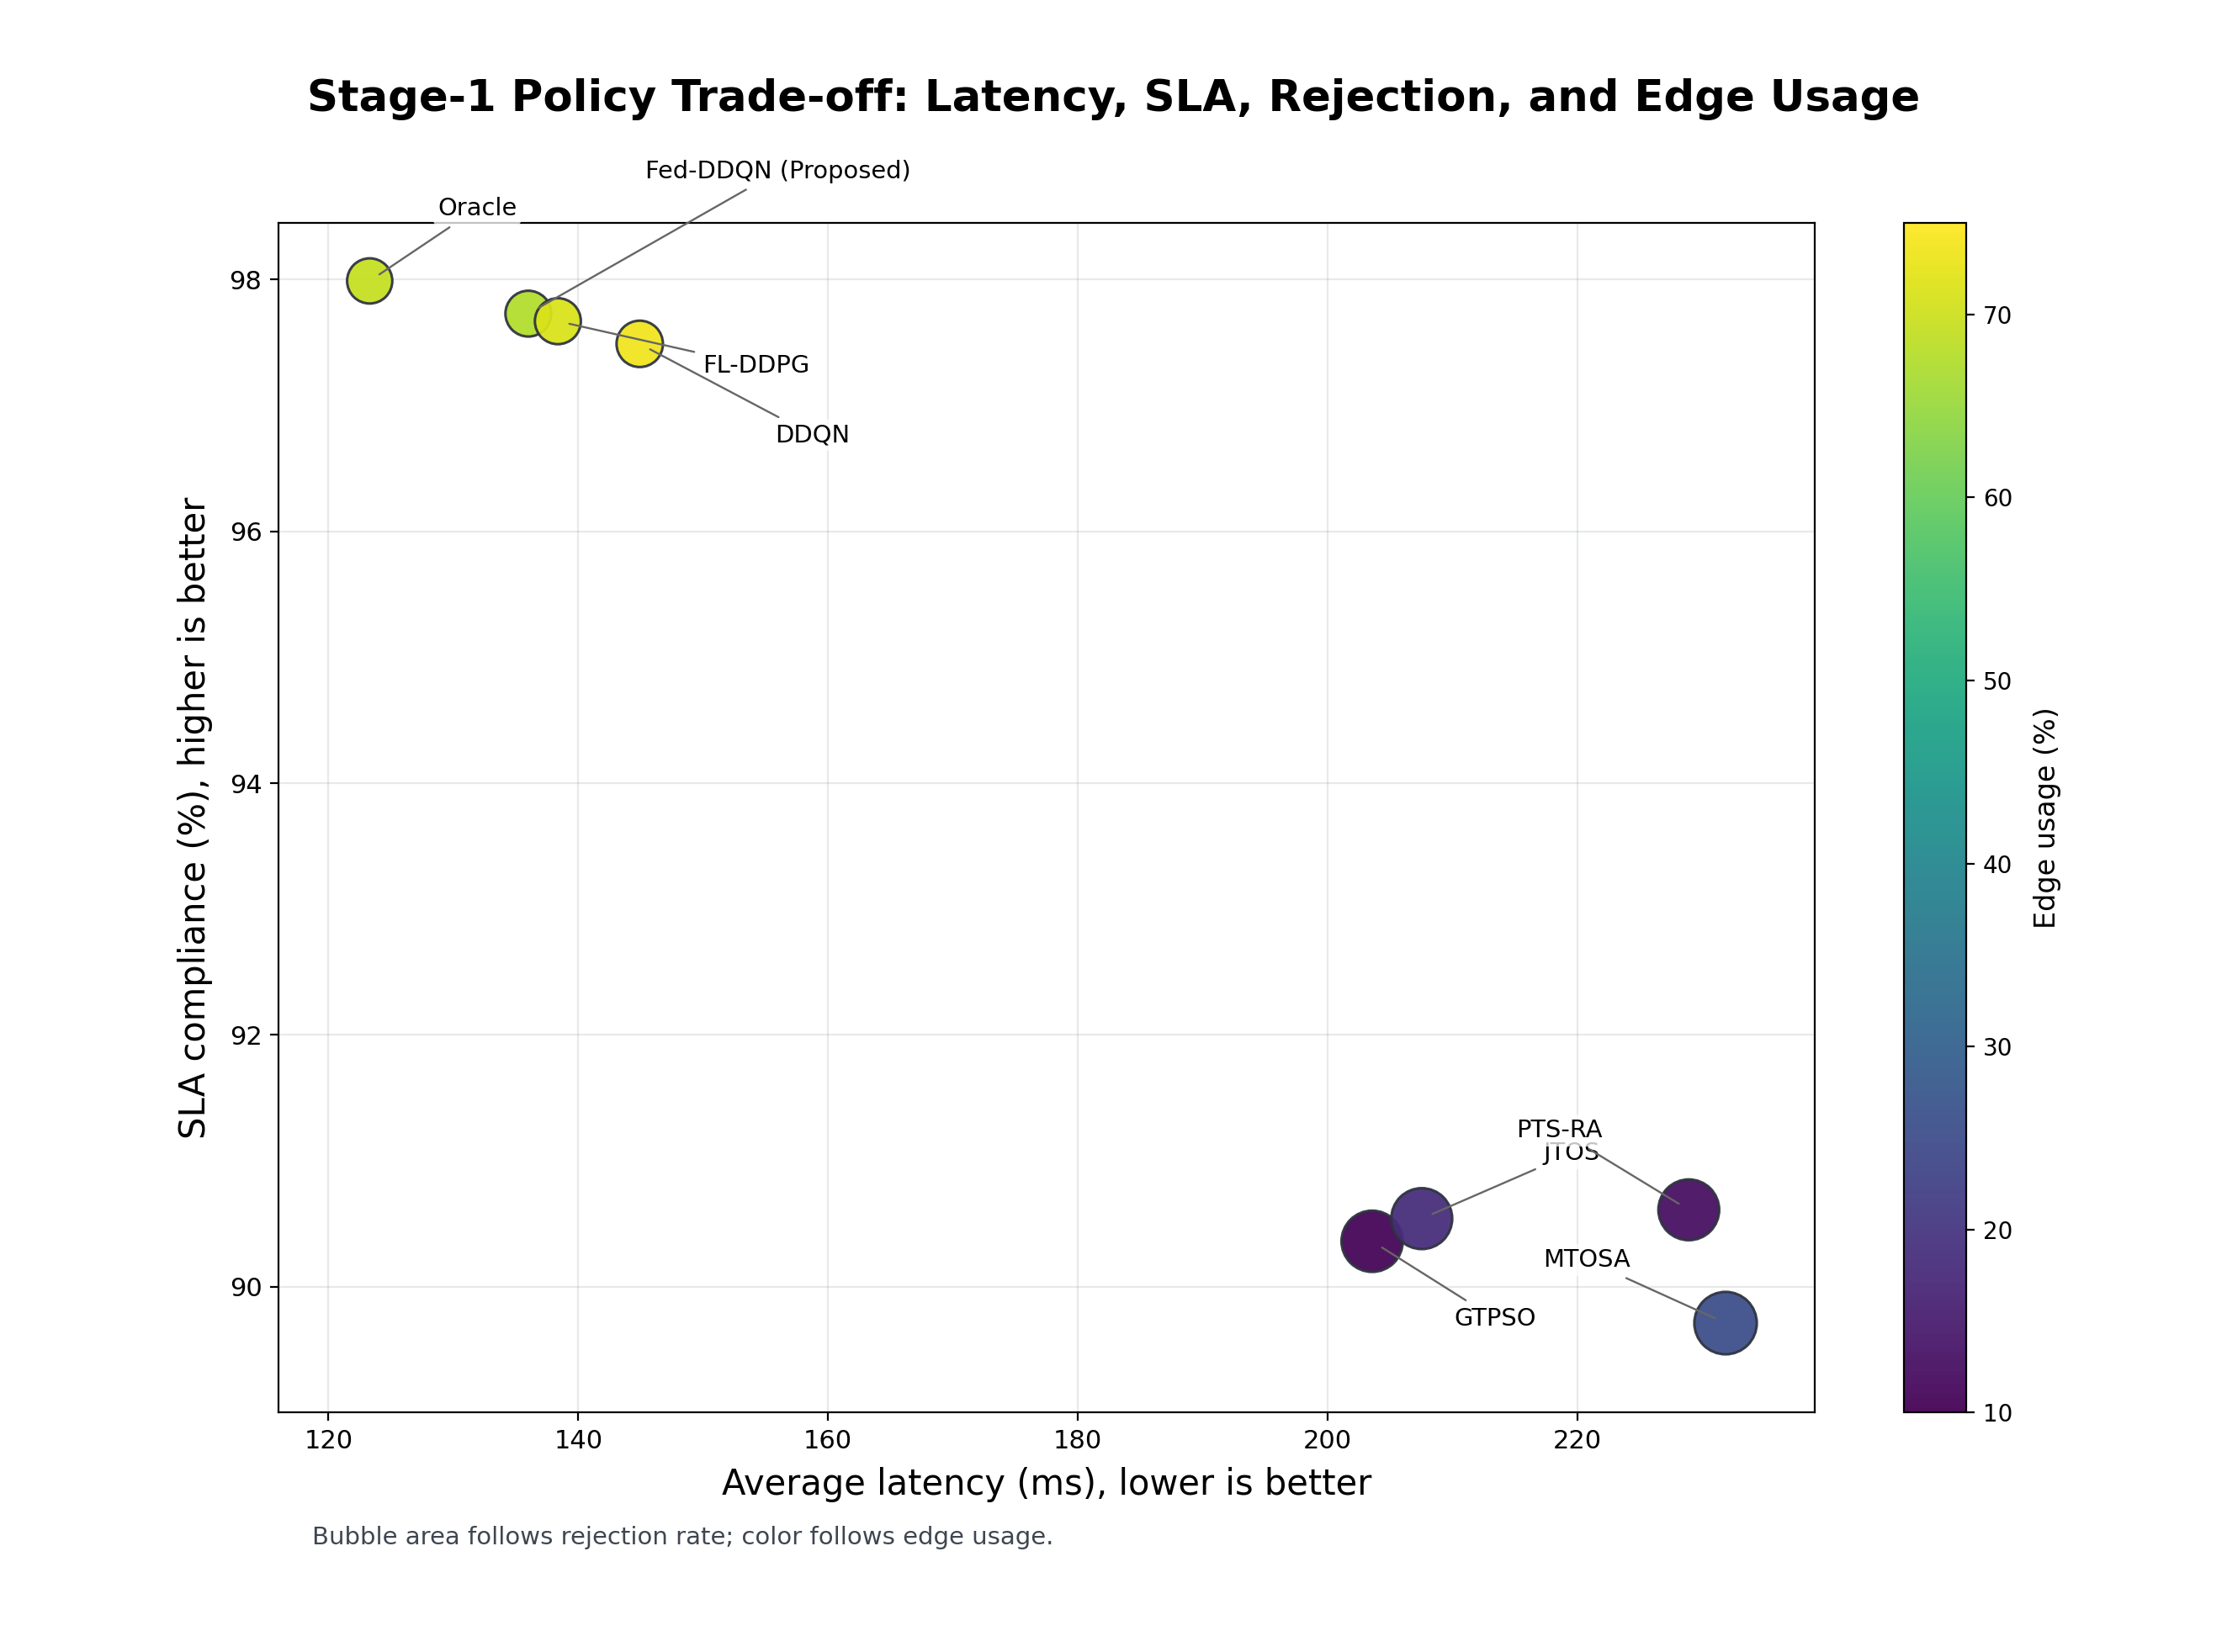
\includegraphics[width=\linewidth]{figures/results/152_fig_a3_policy_tradeoff_bubble.png}
\caption{Stage-1 policy tradeoff among latency, SLA satisfaction, rejection, and edge usage.}
\label{fig:tradeoff_bubble_main}
\end{minipage}\hfill
\begin{minipage}[t]{0.48\textwidth}
\centering
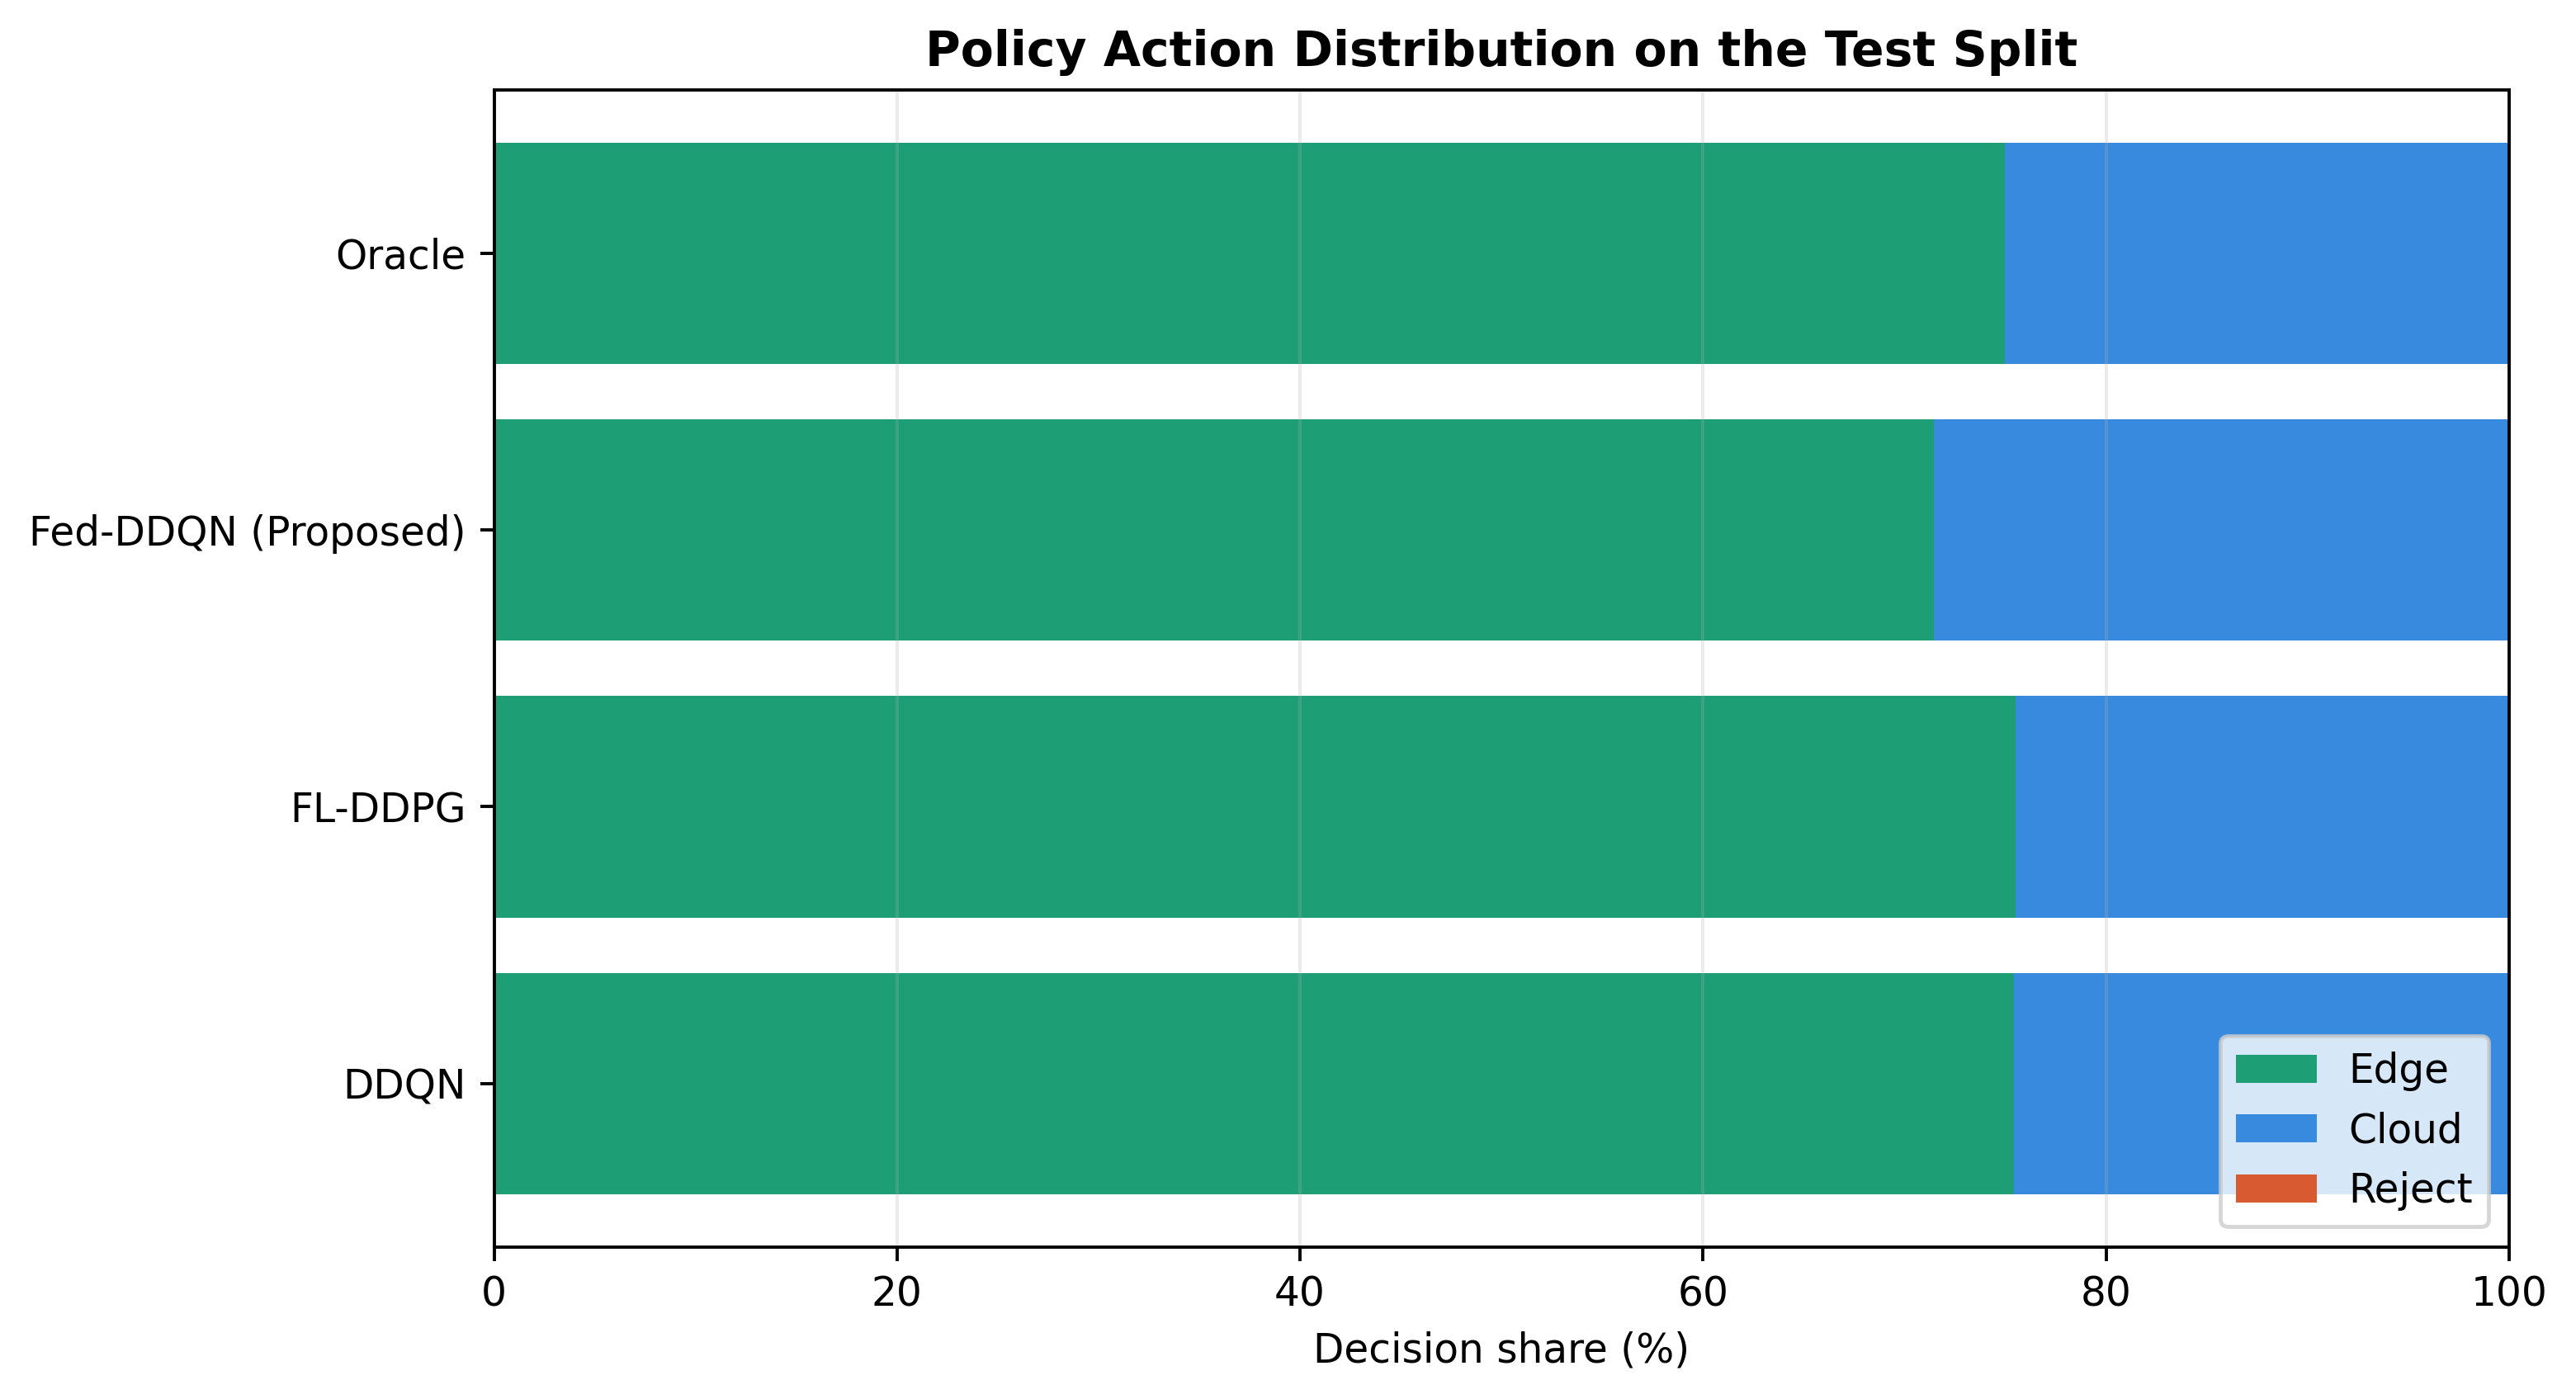
\includegraphics[width=\linewidth]{figures/results/154_fig_a5_policy_action_distribution.png}
\caption{Policy action distribution on the test split for the main comparison methods and the latency-reference Oracle.}
\label{fig:policy_action_distribution}
\end{minipage}
\end{figure*}

Table~\ref{tab:main_results} gives the test-only comparison. The proposed \fedddqn{} achieved \FedLatency{} ms average latency, \FedSLA\% SLA satisfaction, \FedRejection\% rejection, and \FedEdgeUse\% edge usage. It reports the lowest latency among the main comparison methods in the table. Relative to centralized DDQN, latency is lower by \FedVsDDQN\%, which is consistent with the combined effect of the proposed training, reward, and validation design. Relative to the FL-DDPG-style baseline, latency is lower by \FedVsFLDDPG\%, showing that the value-based federated design remains competitive against the implemented federated actor-critic-style comparator.

The latency-reference Oracle reaches \OracleLatency{} ms. It selects the lower finite generated latency among the edge and cloud alternatives and is not a deployable policy. The gap to this latency reference quantifies remaining latency headroom, while the proposed policy moves closer to that reference than the other implemented main comparison methods and maintains low rejection.

\newpage
\begin{figure}[H]
\centering
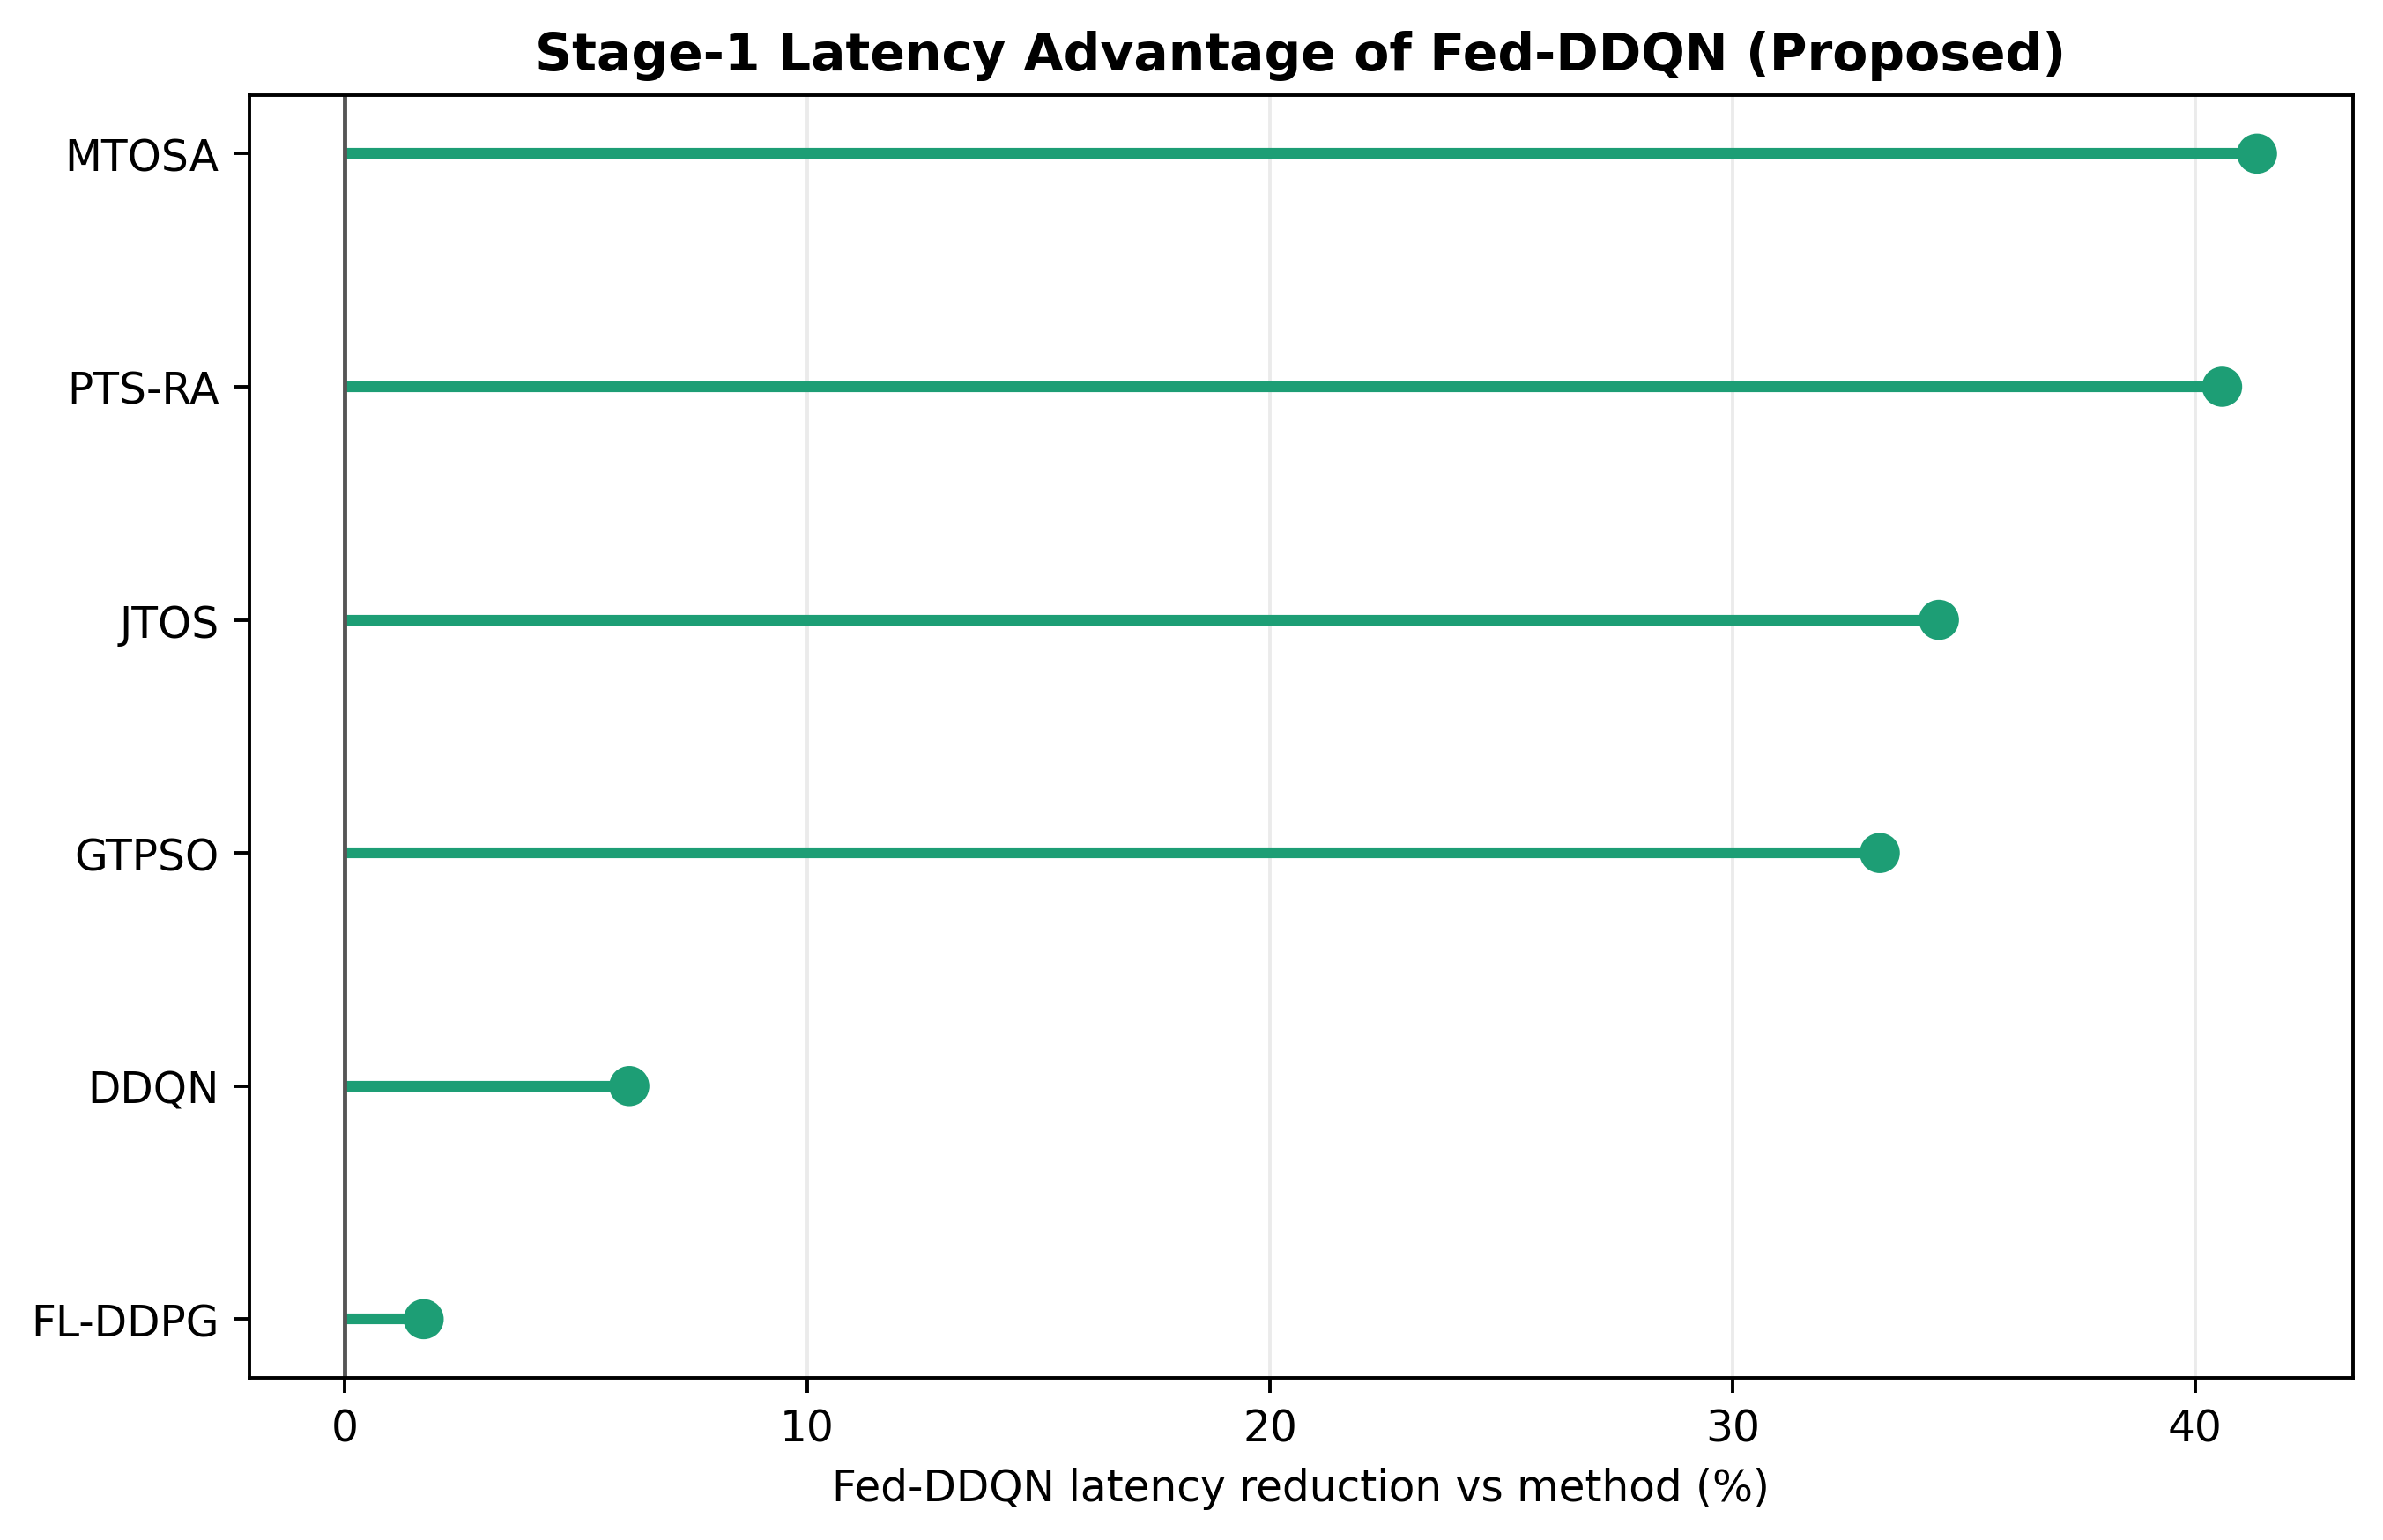
\includegraphics[width=0.92\columnwidth]{figures/results/153_fig_a4_fed_ddqn_latency_improvement.png}
\caption{Average latency comparison between trainable policies and the latency-reference Oracle.}
\label{fig:latency_improvement}
\end{figure}

Figure~\ref{fig:latency_improvement} gives the same result visually. The heuristic and metaheuristic baselines have much higher latency on this dataset because they do not adapt as directly to the generated channel, queue, and fault states. DDQN improves on those rules but remains more edge-heavy than the proposed policy. The proposed method is not simply choosing cloud or edge more often; it uses a more balanced edge share than DDQN and FL-DDPG while preserving the lowest latency among the main comparison methods in Table~\ref{tab:main_results}. Figs.~\ref{fig:tradeoff_bubble_main} and~\ref{fig:policy_action_distribution} show the corresponding tradeoff and routing mix on the held-out test interval.

\begin{figure*}[!t]
\centering
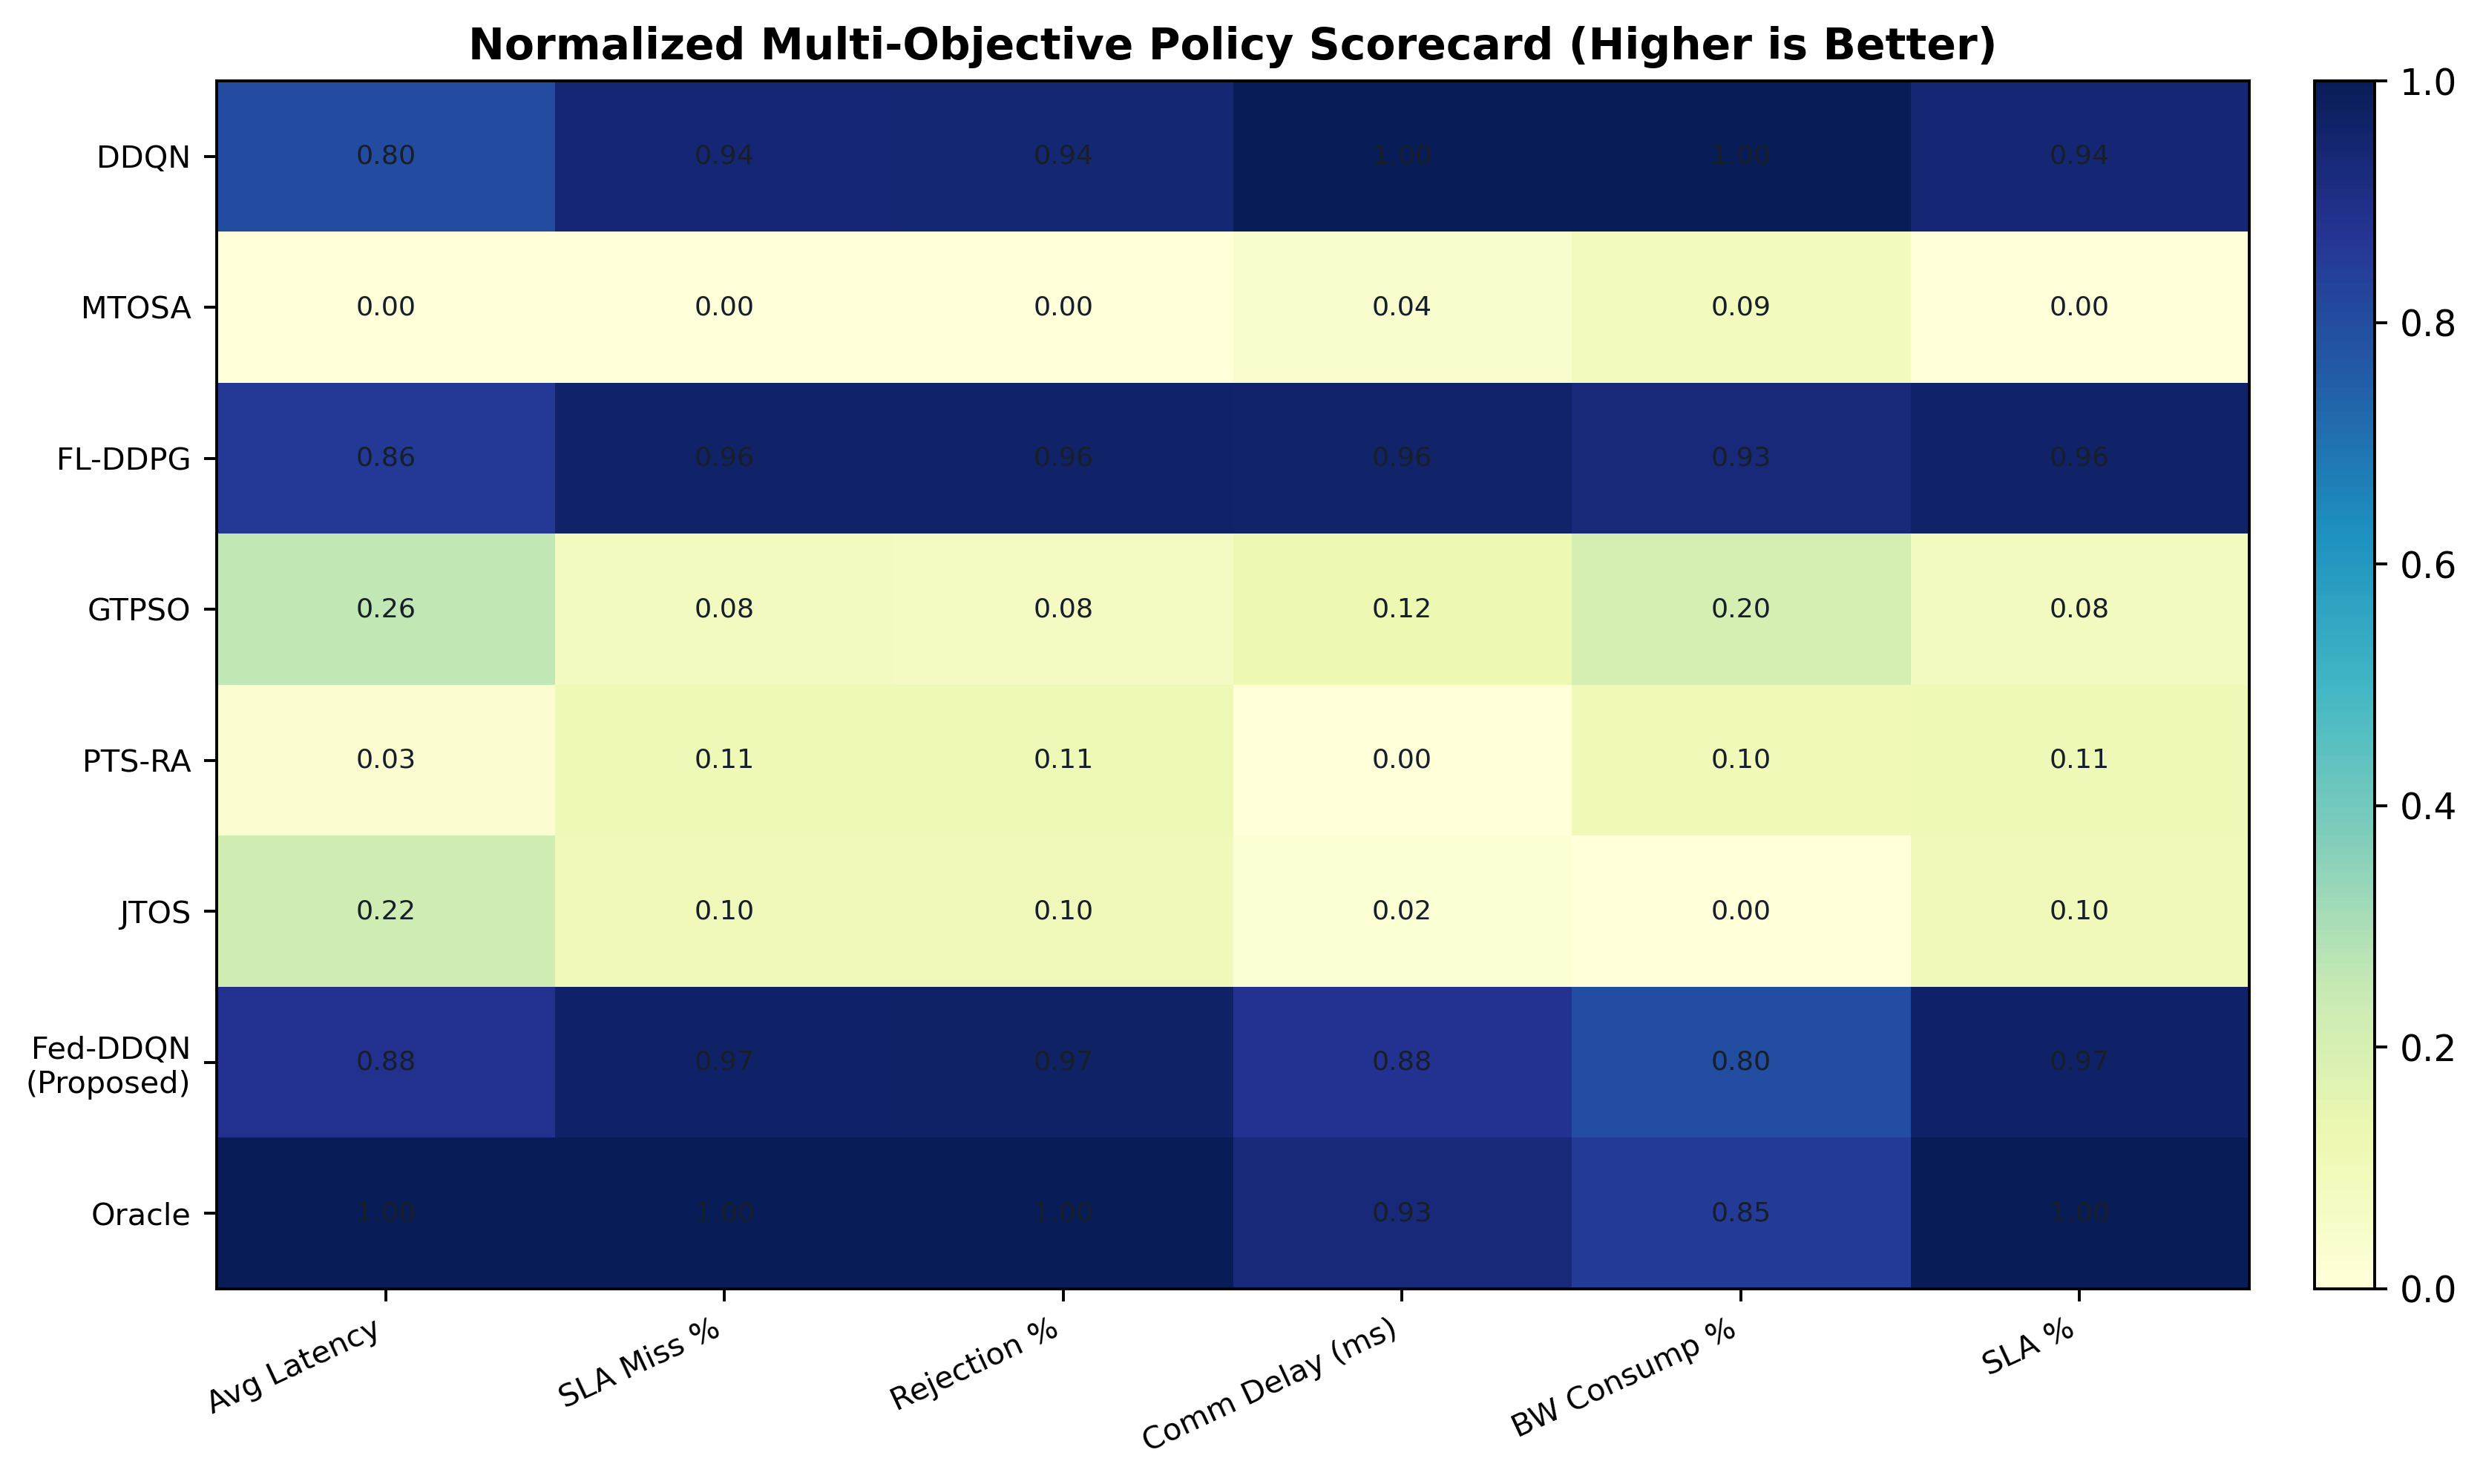
\includegraphics[width=0.72\textwidth]{figures/results/163_fig_a14_policy_multiobjective_scorecard.png}
\caption{Normalized multi-objective policy scorecard. Higher values indicate stronger normalized performance for the corresponding evaluation criterion.}
\label{fig:scorecard}
\end{figure*}
\FloatBarrier

\subsection{QoS and Resource Tradeoff}

The SLA and rejection columns are read alongside latency. A low-latency method would not be useful if it obtained that result by rejecting more tasks or overusing a single destination. The proposed method reports 97.73\% SLA satisfaction and 3.68\% rejection, close to the reported Oracle values of 97.99\% SLA satisfaction and 3.43\% rejection. These Oracle QoS values are descriptive outputs of the latency-reference rule, not guaranteed QoS bounds. The scorecard in Fig.~\ref{fig:scorecard} summarizes this tradeoff.

The edge usage of \fedddqn{} is 67.43\%, while Oracle uses 69.27\%. This alignment suggests that the reward and validation design reduce the edge overuse that can arise in deadline-heavy workloads. The policy still uses edge for many tight-deadline tasks, but it moves cloud-favorable tasks away from overloaded local nodes.

The action-distribution view in Fig.~\ref{fig:policy_action_distribution} is included with the QoS discussion
because edge share is a resource-stability metric. The tradeoff view in Fig.~\ref{fig:tradeoff_bubble_main} shows the same balance against latency and SLA behavior. A policy that lowers latency
by routing nearly everything to edge would be brittle under bursts; the proposed
policy instead stays close to Oracle while keeping rejection low.

\subsection{Scenario Behavior and Oracle Agreement}

Scenario results are reported before the corresponding figures so the reader can follow the argument without losing the thread. Table~\ref{tab:scenario_behavior} uses the same valid held-out policy-evaluation subset as Table~\ref{tab:main_results}, so the scenario counts are not full-benchmark descriptive counts. Together with Fig.~\ref{fig:scenario_diagnostics}, the table indicates that the learned policy does not behave as a one-rule scheduler. Emergency and real-time slices are routed heavily to edge because local execution often dominates when deadlines are tight. AI/video-heavy and firmware slices shift more work toward cloud because they are larger and are often better served by cloud capacity. High edge-queue cases show the cost of local contention, with higher latency and SLA miss despite the same learned policy.

\begin{table}[H]
\centering
\caption{Fed-DDQN scenario behavior on the valid held-out policy-evaluation subset. Scenario subsets are test/evaluation slices and may overlap.}
\label{tab:scenario_behavior}
\scriptsize
\setlength{\tabcolsep}{2.4pt}
\resizebox{\columnwidth}{!}{%
\begin{tabular}{@{}p{0.30\columnwidth}rrrr@{}}
\toprule
Scenario & $N$ & Avg. lat. & SLA miss & Edge use \\
\midrule
All valid rows & 9733 & 136.855 $\pm$ 0.599 & 2.29 $\pm$ 0.05 & 67.56 $\pm$ 0.37 \\
Normal traffic & 4061 & 70.914 $\pm$ 0.204 & 0.26 $\pm$ 0.01 & 67.56 $\pm$ 0.33 \\
Congestion & 5672 & 184.066 $\pm$ 0.923 & 3.75 $\pm$ 0.09 & 67.56 $\pm$ 0.86 \\
Jitter storm & 447 & 199.934 $\pm$ 0.952 & 2.98 $\pm$ 0.10 & 87.47 $\pm$ 0.73 \\
High edge queue & 845 & 245.461 $\pm$ 2.105 & 11.05 $\pm$ 0.31 & 58.50 $\pm$ 2.54 \\
Emergency & 492 & 34.049 $\pm$ 1.146 & 22.76 $\pm$ 0.17 & 99.19 $\pm$ 0.60 \\
Real-time & 4130 & 43.251 $\pm$ 0.319 & 5.40 $\pm$ 0.12 & 98.41 $\pm$ 0.38 \\
Low battery & 958 & 144.930 $\pm$ 1.125 & 3.44 $\pm$ 0.09 & 66.81 $\pm$ 1.20 \\
AI/video-heavy & 1640 & 282.075 $\pm$ 2.893 & 0.00 $\pm$ 0.00 & 21.44 $\pm$ 0.42 \\
Firmware & 251 & 252.343 $\pm$ 2.179 & 0.00 $\pm$ 0.00 & 33.73 $\pm$ 2.73 \\
\bottomrule
\end{tabular}}
\begin{minipage}{0.96\columnwidth}
\vspace{0.2em}
\scriptsize\emph{Note:} Values are mean $\pm$ standard deviation across the three Fed-DDQN seeds exported for the manuscript. The raw temporal test split contains 11,957 rows; the policy-evaluation subset used for Table~\ref{tab:main_results} contains 9,733 rows after valid generated-latency filtering. Scenario slices are drawn from that valid held-out subset.
\end{minipage}
\end{table}


\begin{figure*}[!t]
\centering
\begin{minipage}[t]{0.48\textwidth}
\centering
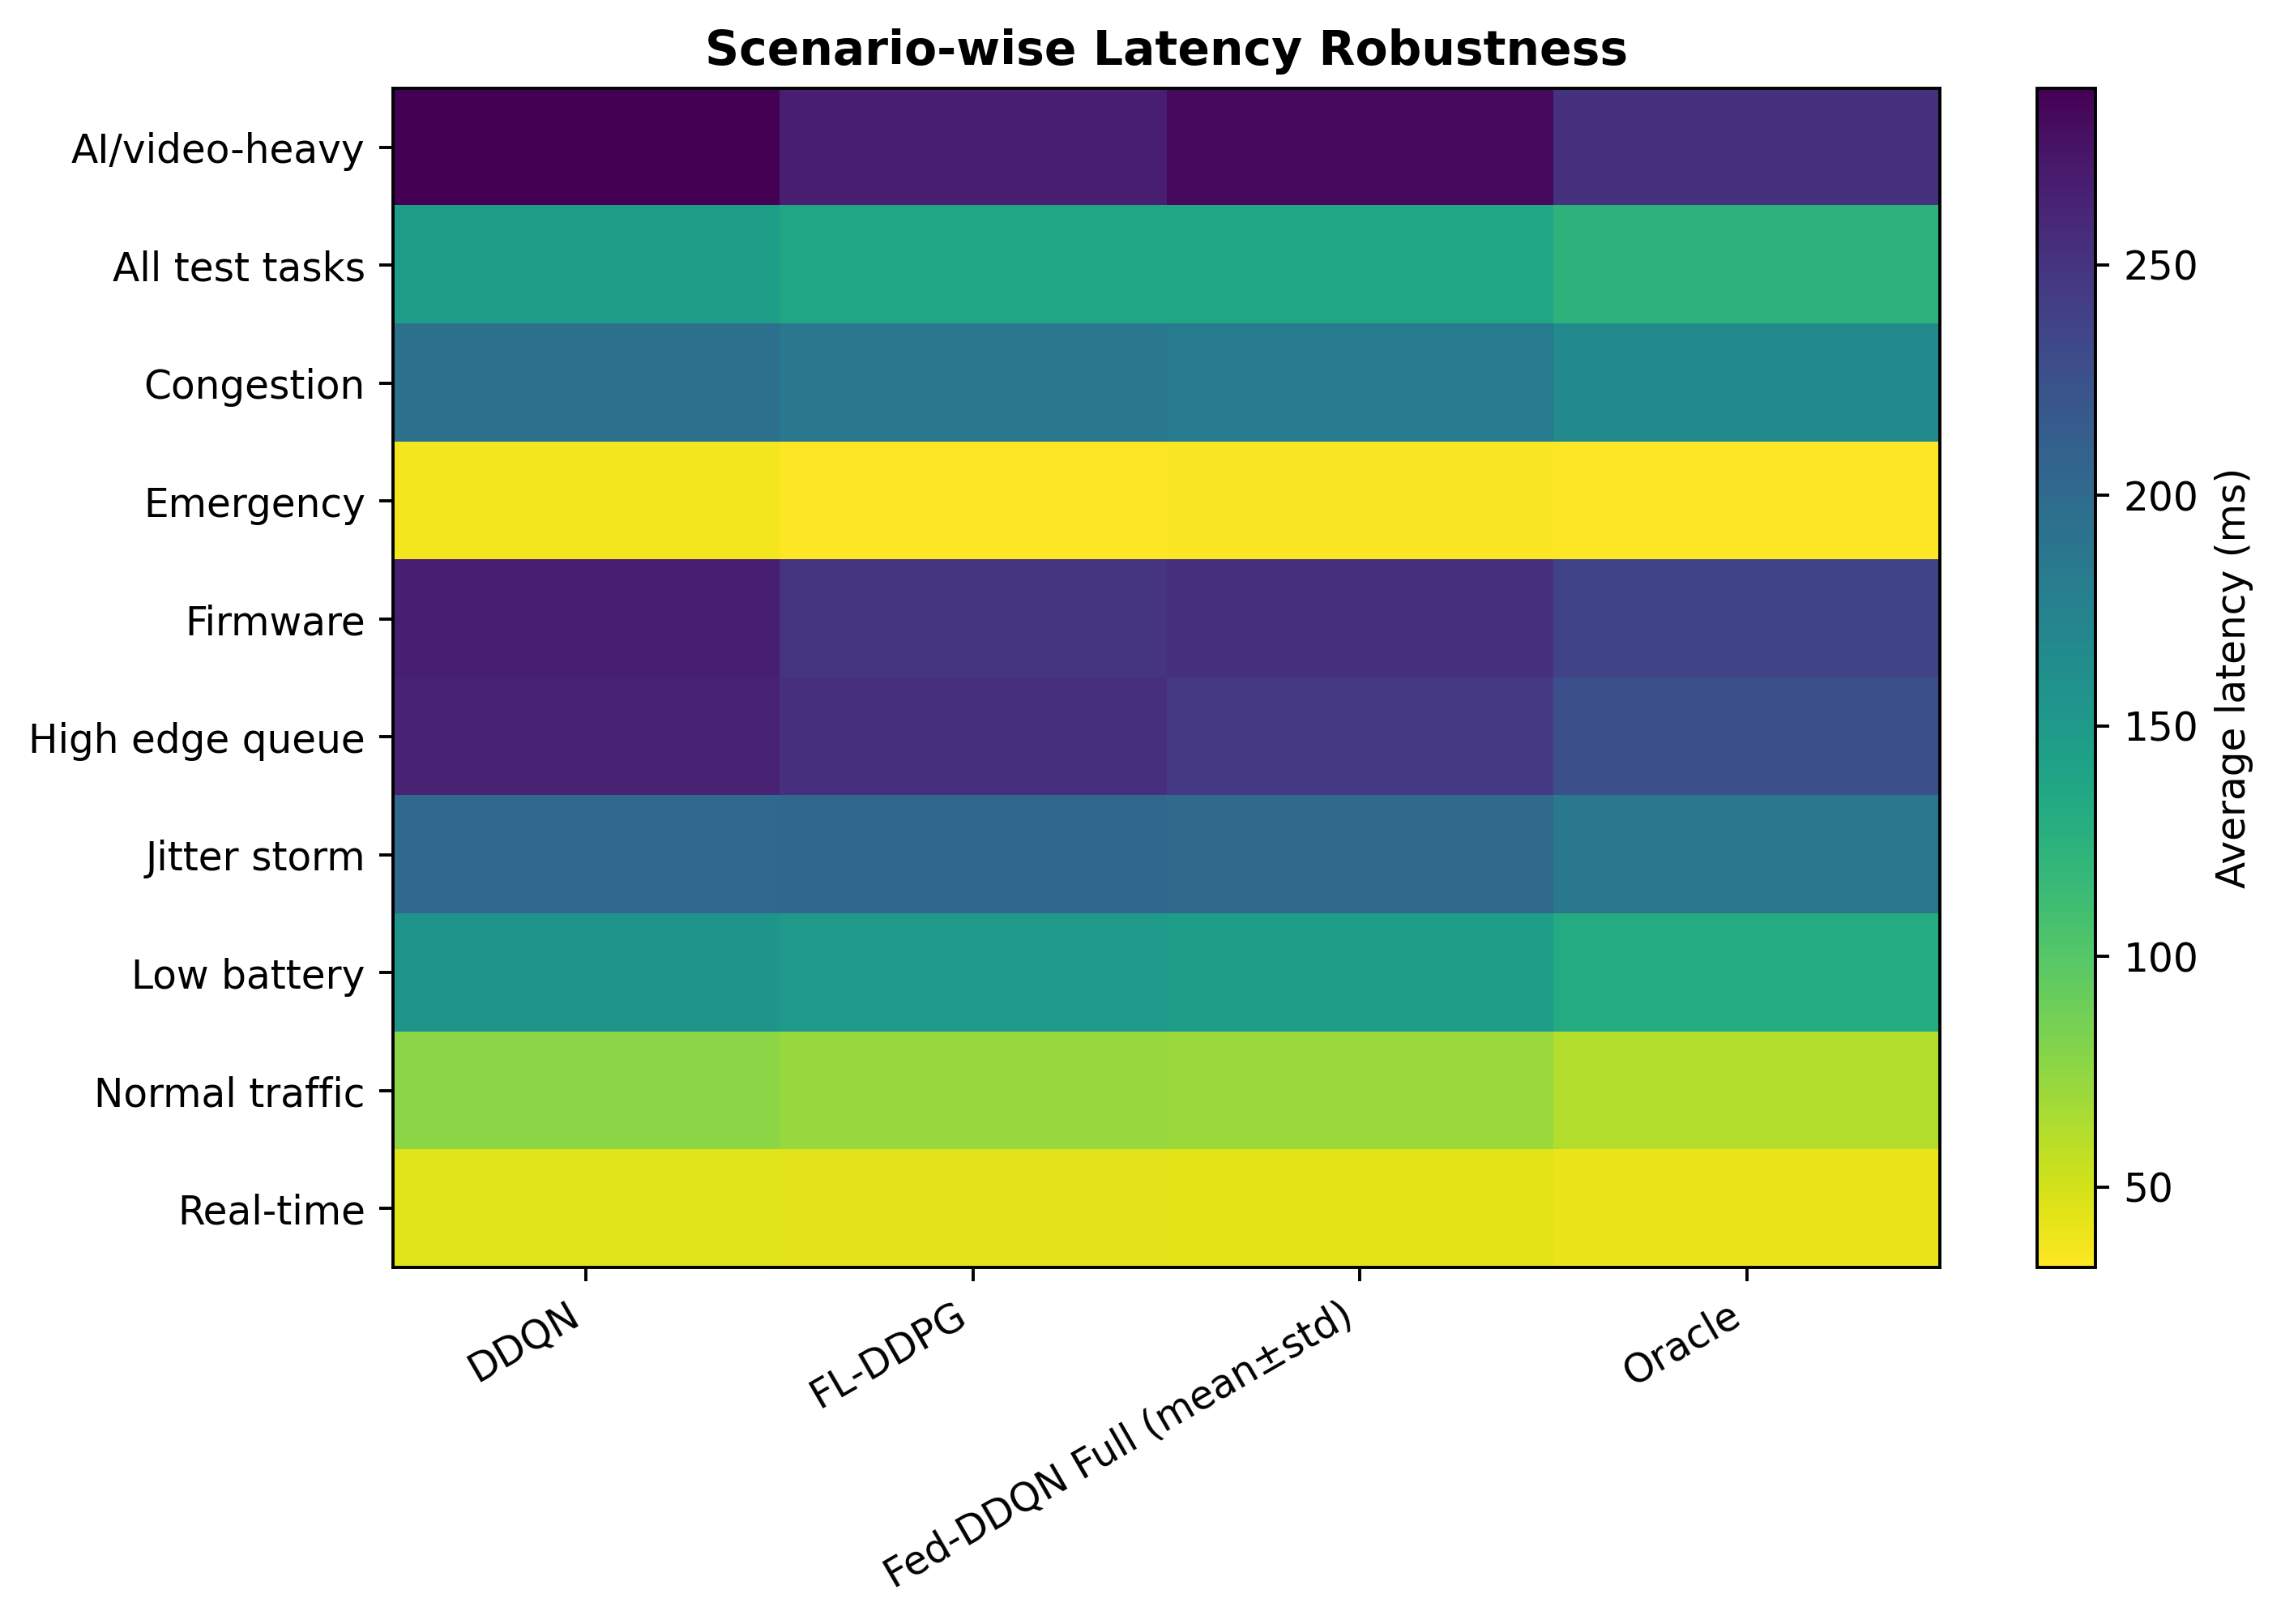
\includegraphics[width=\linewidth]{figures/results/155_fig_a6_scenario_latency_heatmap.png}
\small (a) Scenario latency
\end{minipage}\hfill
\begin{minipage}[t]{0.48\textwidth}
\centering
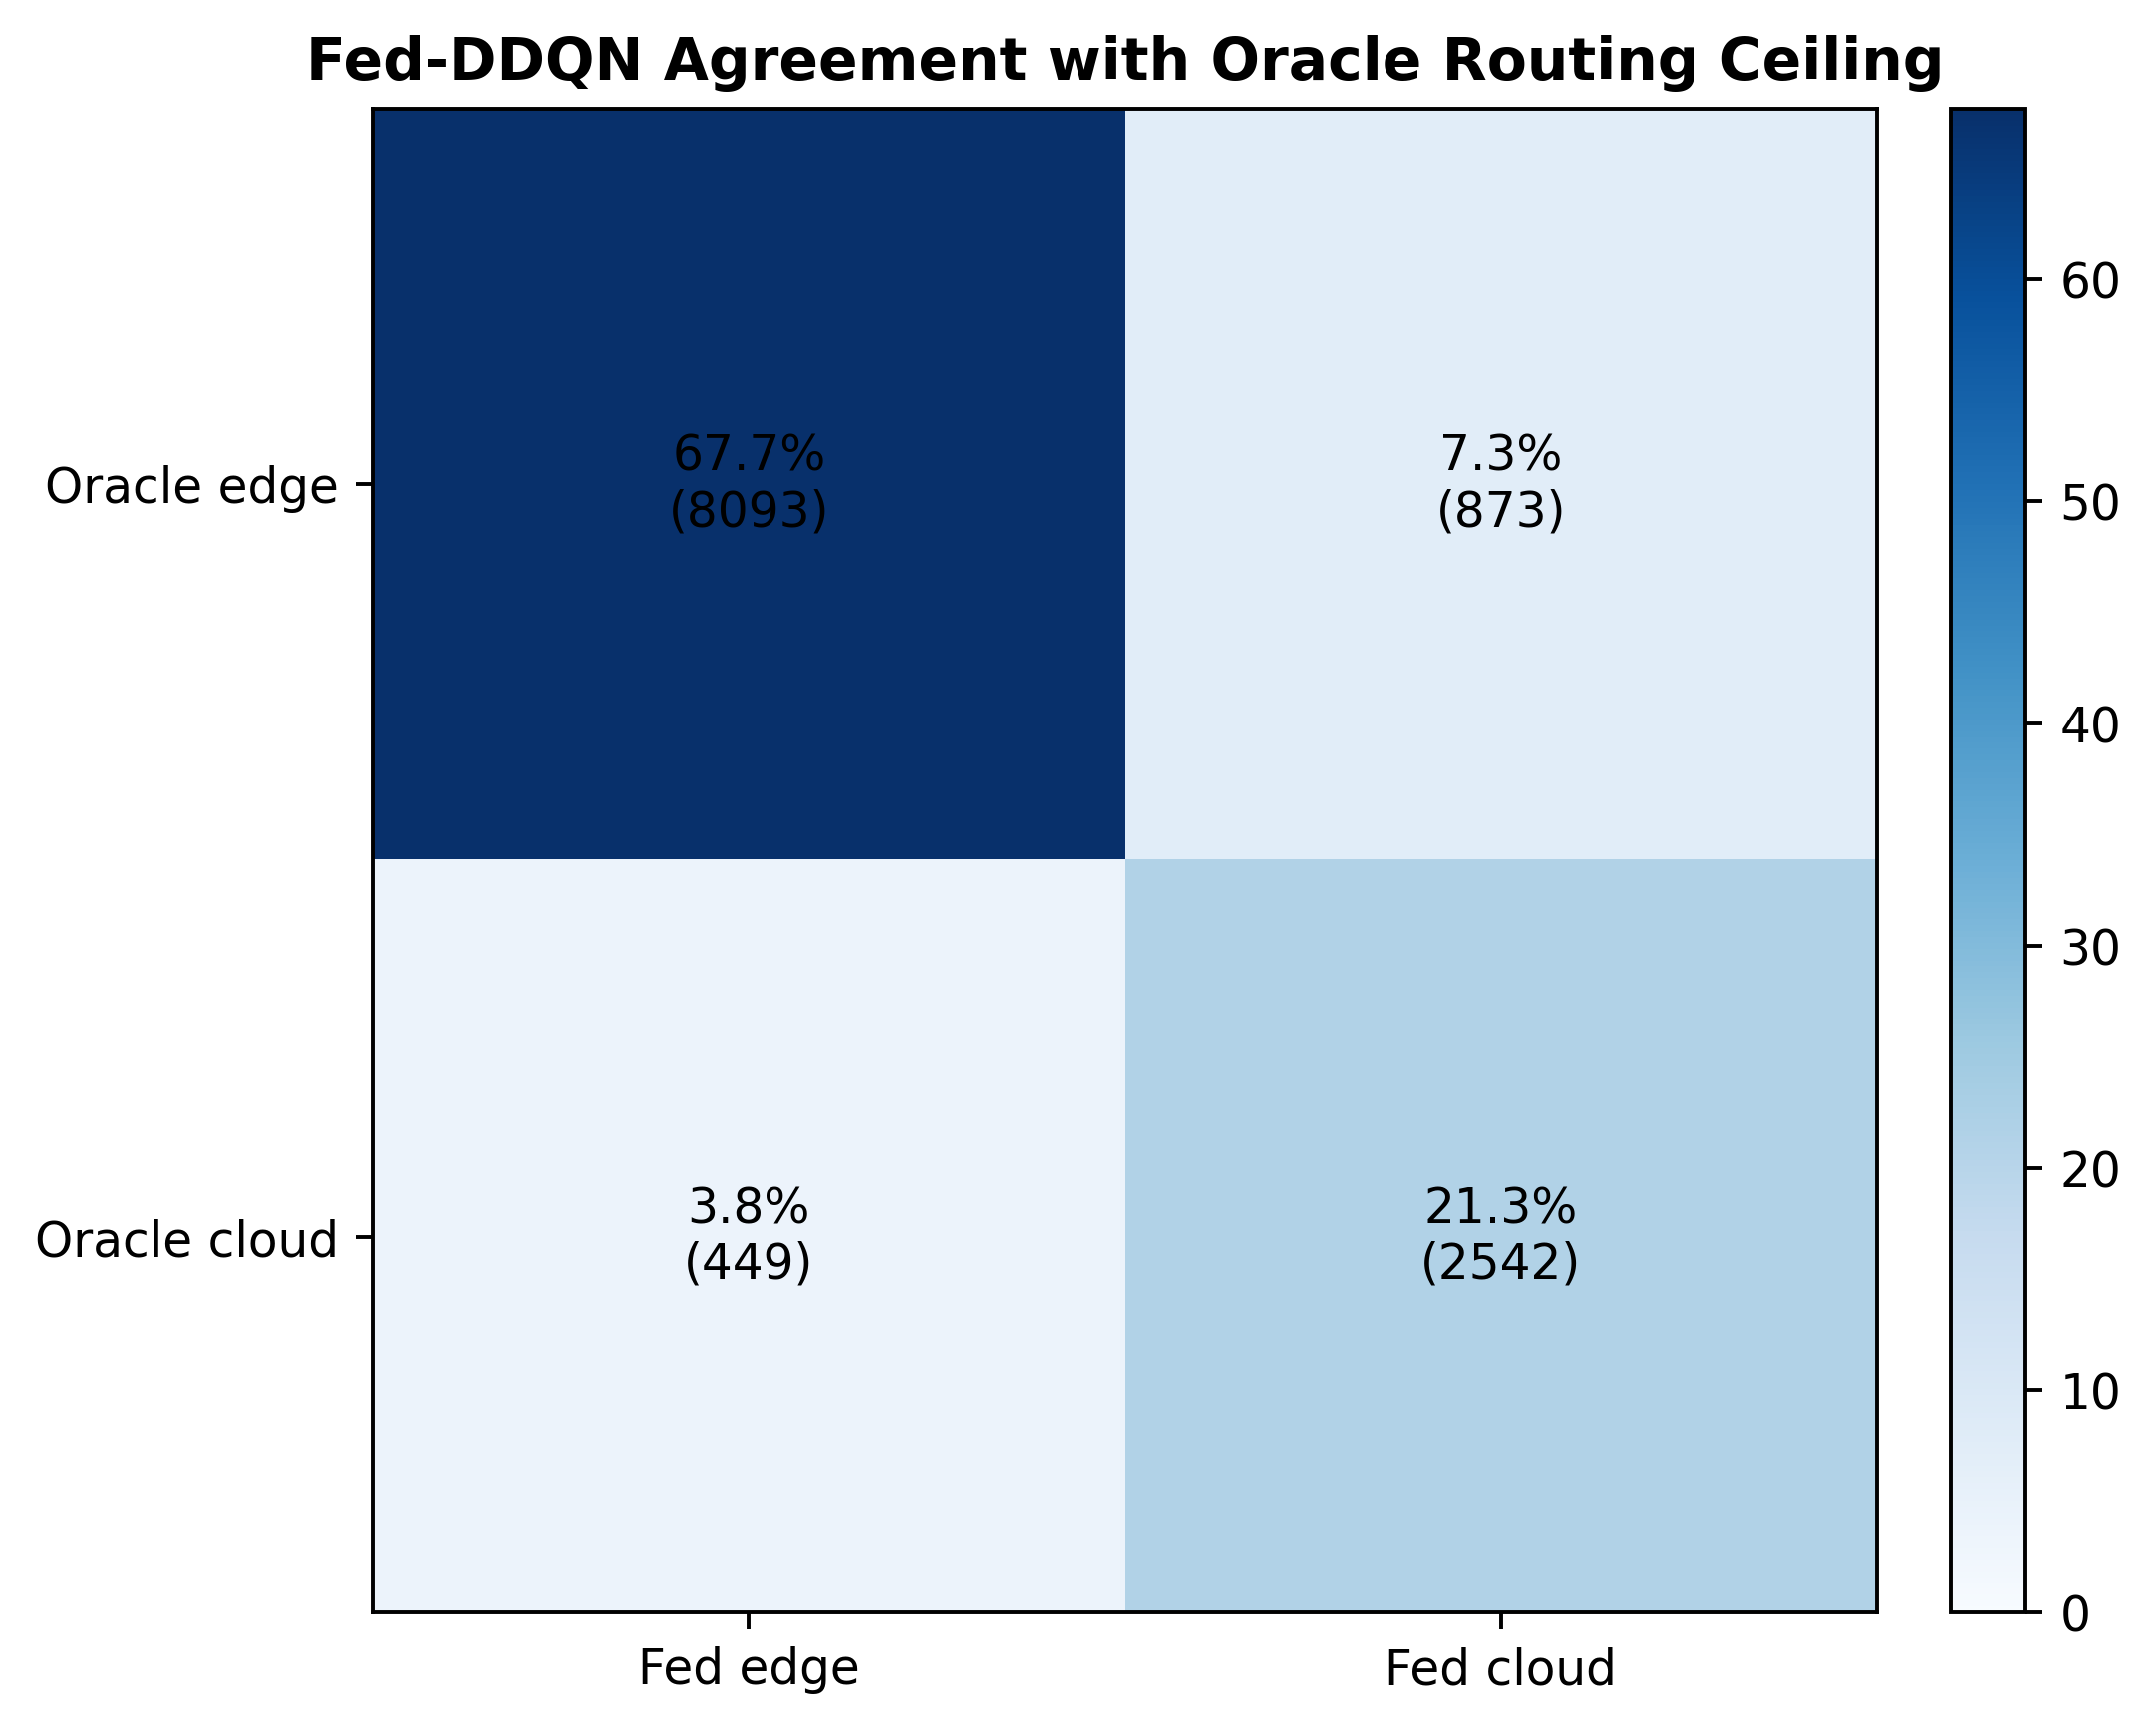
\includegraphics[width=\linewidth]{figures/diagnostics/164_fig_a15_fed_oracle_agreement_matrix.png}
\small (b) Oracle agreement
\end{minipage}
\par\smallskip
\begin{minipage}[t]{0.52\textwidth}
\centering
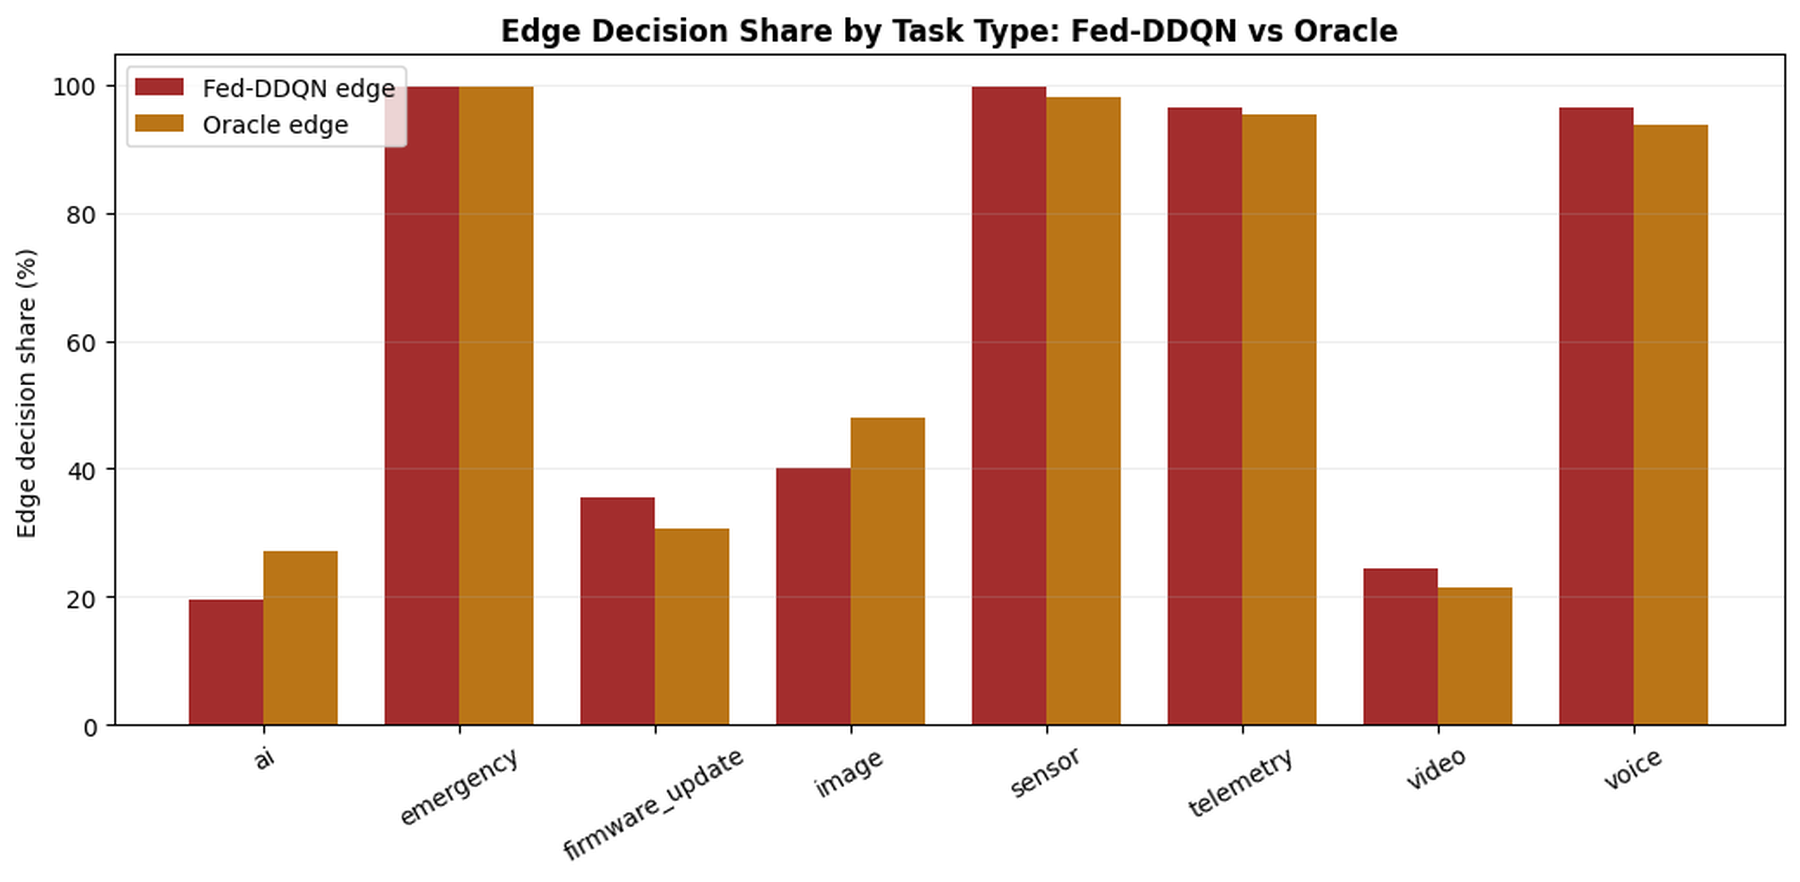
\includegraphics[width=\linewidth]{figures/diagnostics/172_fig_a25_task_type_edge_share.png}
\small (c) Task-type edge share
\end{minipage}
\caption{Scenario diagnostics for the proposed policy. Panel (a) compares latency across workload slices, panel (b) shows agreement with the latency-reference Oracle, and panel (c) compares task-type edge decisions with Oracle.}
\label{fig:scenario_diagnostics}
\end{figure*}
\FloatBarrier

The Oracle-agreement panel in Fig.~\ref{fig:scenario_diagnostics} is a diagnostic rather than a primary score. It identifies where the learned policy still disagrees with the generated latency reference. Disagreement on ambiguous tasks is not automatically wrong, because many cases have similar edge and cloud latency. Disagreement on heavy tasks or emergency tasks matters more because the cost of the wrong destination is larger.

\subsection{Multi-Seed Ablation}

The multi-seed result reports \MultiSeedLatency{} $\pm$ \MultiSeedLatencySD{} ms for the proposed configuration across seeds 42, 77, and 123. The low standard deviation indicates stable behavior across the evaluated seeds. The ablations are close in latency, which is expected because the design objective is not latency alone. The action-aware pressure variant has a slightly lower mean latency in the ablation table, while other variants trade latency, rejection, SLA, and edge usage differently. The proposed configuration is retained because it is selected by the balanced validation objective and gives a more controlled edge-usage pattern.

\begin{table*}[!t]
\centering
\caption{Three-seed Fed-DDQN and ablation summary.}
\label{tab:multiseed_ablation}
\small
\setlength{\tabcolsep}{5pt}
\renewcommand{\arraystretch}{1.08}
\begin{tabular*}{0.96\textwidth}{@{\extracolsep{\fill}}lcccc@{}}
\toprule
Variant & Avg. latency (ms) & SLA (\%) & Rejection (\%) & Edge usage (\%) \\
\midrule
\fedddqn{} Proposed & $136.855 \pm 0.599$ & $97.71 \pm 0.05$ & $3.70 \pm 0.06$ & $67.56 \pm 0.37$ \\
\fedddqn{} + Prioritized Replay & $137.221 \pm 1.089$ & $97.64 \pm 0.06$ & $3.77 \pm 0.06$ & $66.04 \pm 0.33$ \\
\fedddqn{} + Action-Aware Pressure & $136.393 \pm 0.896$ & $97.68 \pm 0.07$ & $3.73 \pm 0.07$ & $67.50 \pm 1.53$ \\
\fedddqn{} without FedProx & $136.495 \pm 0.272$ & $97.65 \pm 0.10$ & $3.77 \pm 0.10$ & $67.07 \pm 1.11$ \\
\fedddqn{} with Hard Target Update & $137.266 \pm 0.501$ & $97.71 \pm 0.05$ & $3.70 \pm 0.04$ & $67.98 \pm 1.08$ \\
\fedddqn{} without Heavy-Task Penalty & $136.845 \pm 0.498$ & $97.68 \pm 0.06$ & $3.73 \pm 0.05$ & $66.99 \pm 2.34$ \\
\bottomrule
\end{tabular*}
\par\smallskip
\begin{minipage}{0.94\textwidth}
\footnotesize Values are three-seed means with standard deviations from the completed Fed-DDQN ablation export.
\end{minipage}
\end{table*}

\FloatBarrier

\begin{figure}[H]
\centering
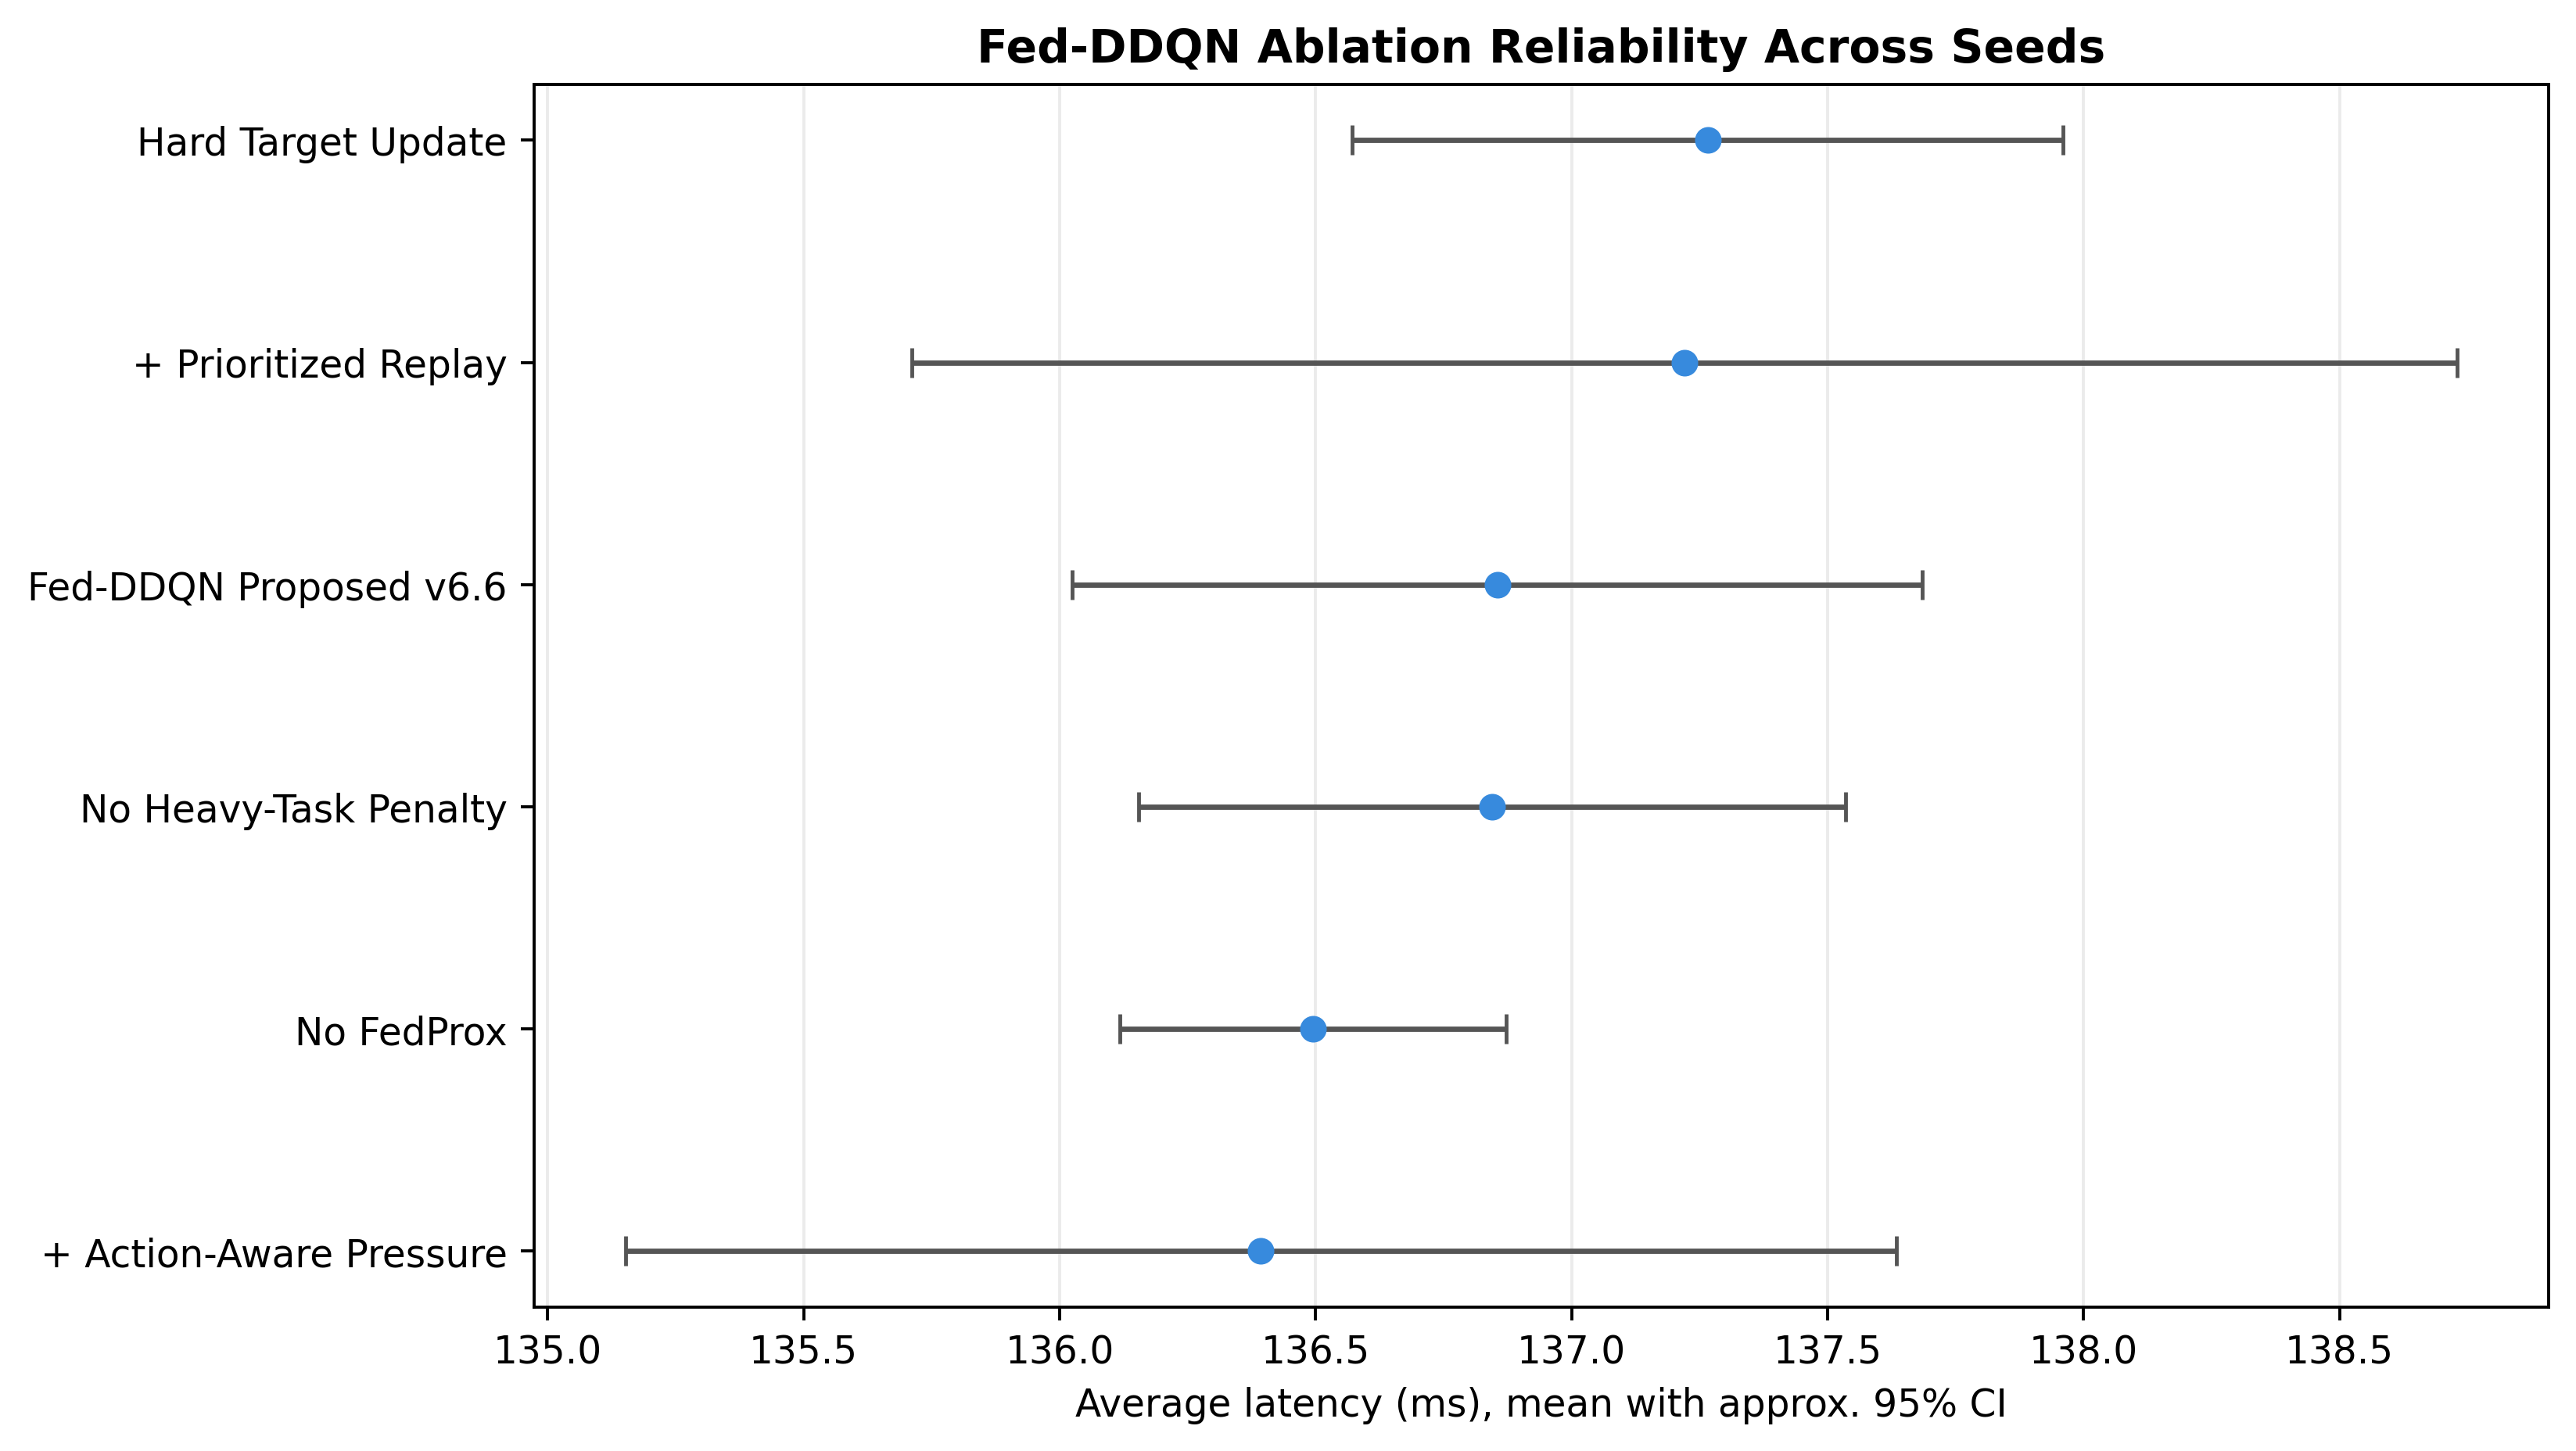
\includegraphics[width=0.92\columnwidth]{figures/diagnostics/156_fig_a7_multiseed_ablation_latency_ci.png}
\caption{Three-seed latency intervals for the proposed configuration and ablations.}
\label{fig:ablation_ci}
\end{figure}

The ablation results support the proposed configuration as a balanced design. Rather than optimizing a single scalar in isolation, the final model balances latency, rejection, SLA satisfaction, and destination usage.

\FloatBarrier
\subsection{Resource Allocation}

The allocator results explain what happens after the Stage-1 policy selects edge execution. The offloading policy decides where the task goes. The allocator decides how much edge resource to assign after edge is selected. In Table~\ref{tab:allocator_results}, the raw residual allocator reports 0.0504 proxy-target MAE, capacity normalization removes the capacity-violation problem, and the residual plus risk-projection variant reaches 0.0204 proxy-target MAE with zero capacity violation. In the broader comparison, the hand-designed rejection-aware demand rule gives the lowest MAE, while the residual plus risk-projection variant gives the best proxy-target efficiency score, 89.295, the lowest under-allocation, and zero capacity violation.

The raw residual allocator has a notable weakness: it can reduce local error but violate capacity. Capacity normalization fixes that. Risk projection further reduces under-allocation for tasks with higher deadline pressure or QoS/admission risk. The resulting resource manager is more defensible than a pure neural output because the final allocation remains constrained by node capacity.

\begin{figure}[H]
\centering
\scriptsize
\setlength{\fboxsep}{5pt}
\fbox{\begin{minipage}{0.88\columnwidth}
\textbf{Stage-2 allocation readout.}
\[
\begin{aligned}
\tilde{\mathbf{y}}_i =
\mathbf{b}_i +
f_{\phi}(\mathbf{z}_i),\\
\mathbf{y}^{\mathrm{res}}_i =
\Pi_{\mathrm{cap}}\!\left(\mathrm{clip}_{[0,1]}(\tilde{\mathbf{y}}_i)\right),\\
\mathbf{y}^{\mathrm{dem}}_i =
\Pi_{\mathrm{cap}}\!\left(\omega_i\mathbf{d}^{\mathrm{raw}}_i\right),\\
\mathbf{y}_i^{risk} =
\Pi_{\mathrm{cap}}\!\left(
0.10\mathbf{y}^{\mathrm{res}}_i+
0.90\mathbf{y}^{\mathrm{dem}}_i
\right),\\
\hat{\mathbf{y}}_i =
\Pi_{\mathrm{cap}}\!\left(\mathbf{y}_i^{risk}\right).
\end{aligned}
\]
Here $\mathbf{b}_i$ is the demand-proportional base, $\tilde{\mathbf{y}}_i$ is the residual-corrected allocation, $\mathbf{y}^{\mathrm{res}}_i$ is the capacity-normalized residual branch, $\mathbf{y}^{\mathrm{dem}}_i$ is the rejection-aware demand branch, $\mathbf{y}_i^{risk}$ is the blended risk-projected allocation, and $\hat{\mathbf{y}}_i$ is the final capacity-normalized assignment.
\end{minipage}}
\caption{Capacity-aware interpretation of the rejection-aware residual allocator using the same Stage-2 target and prediction notation as the allocator equations.}
\label{fig:allocator_projection_readout}
\end{figure}

\begin{figure}[H]
\centering
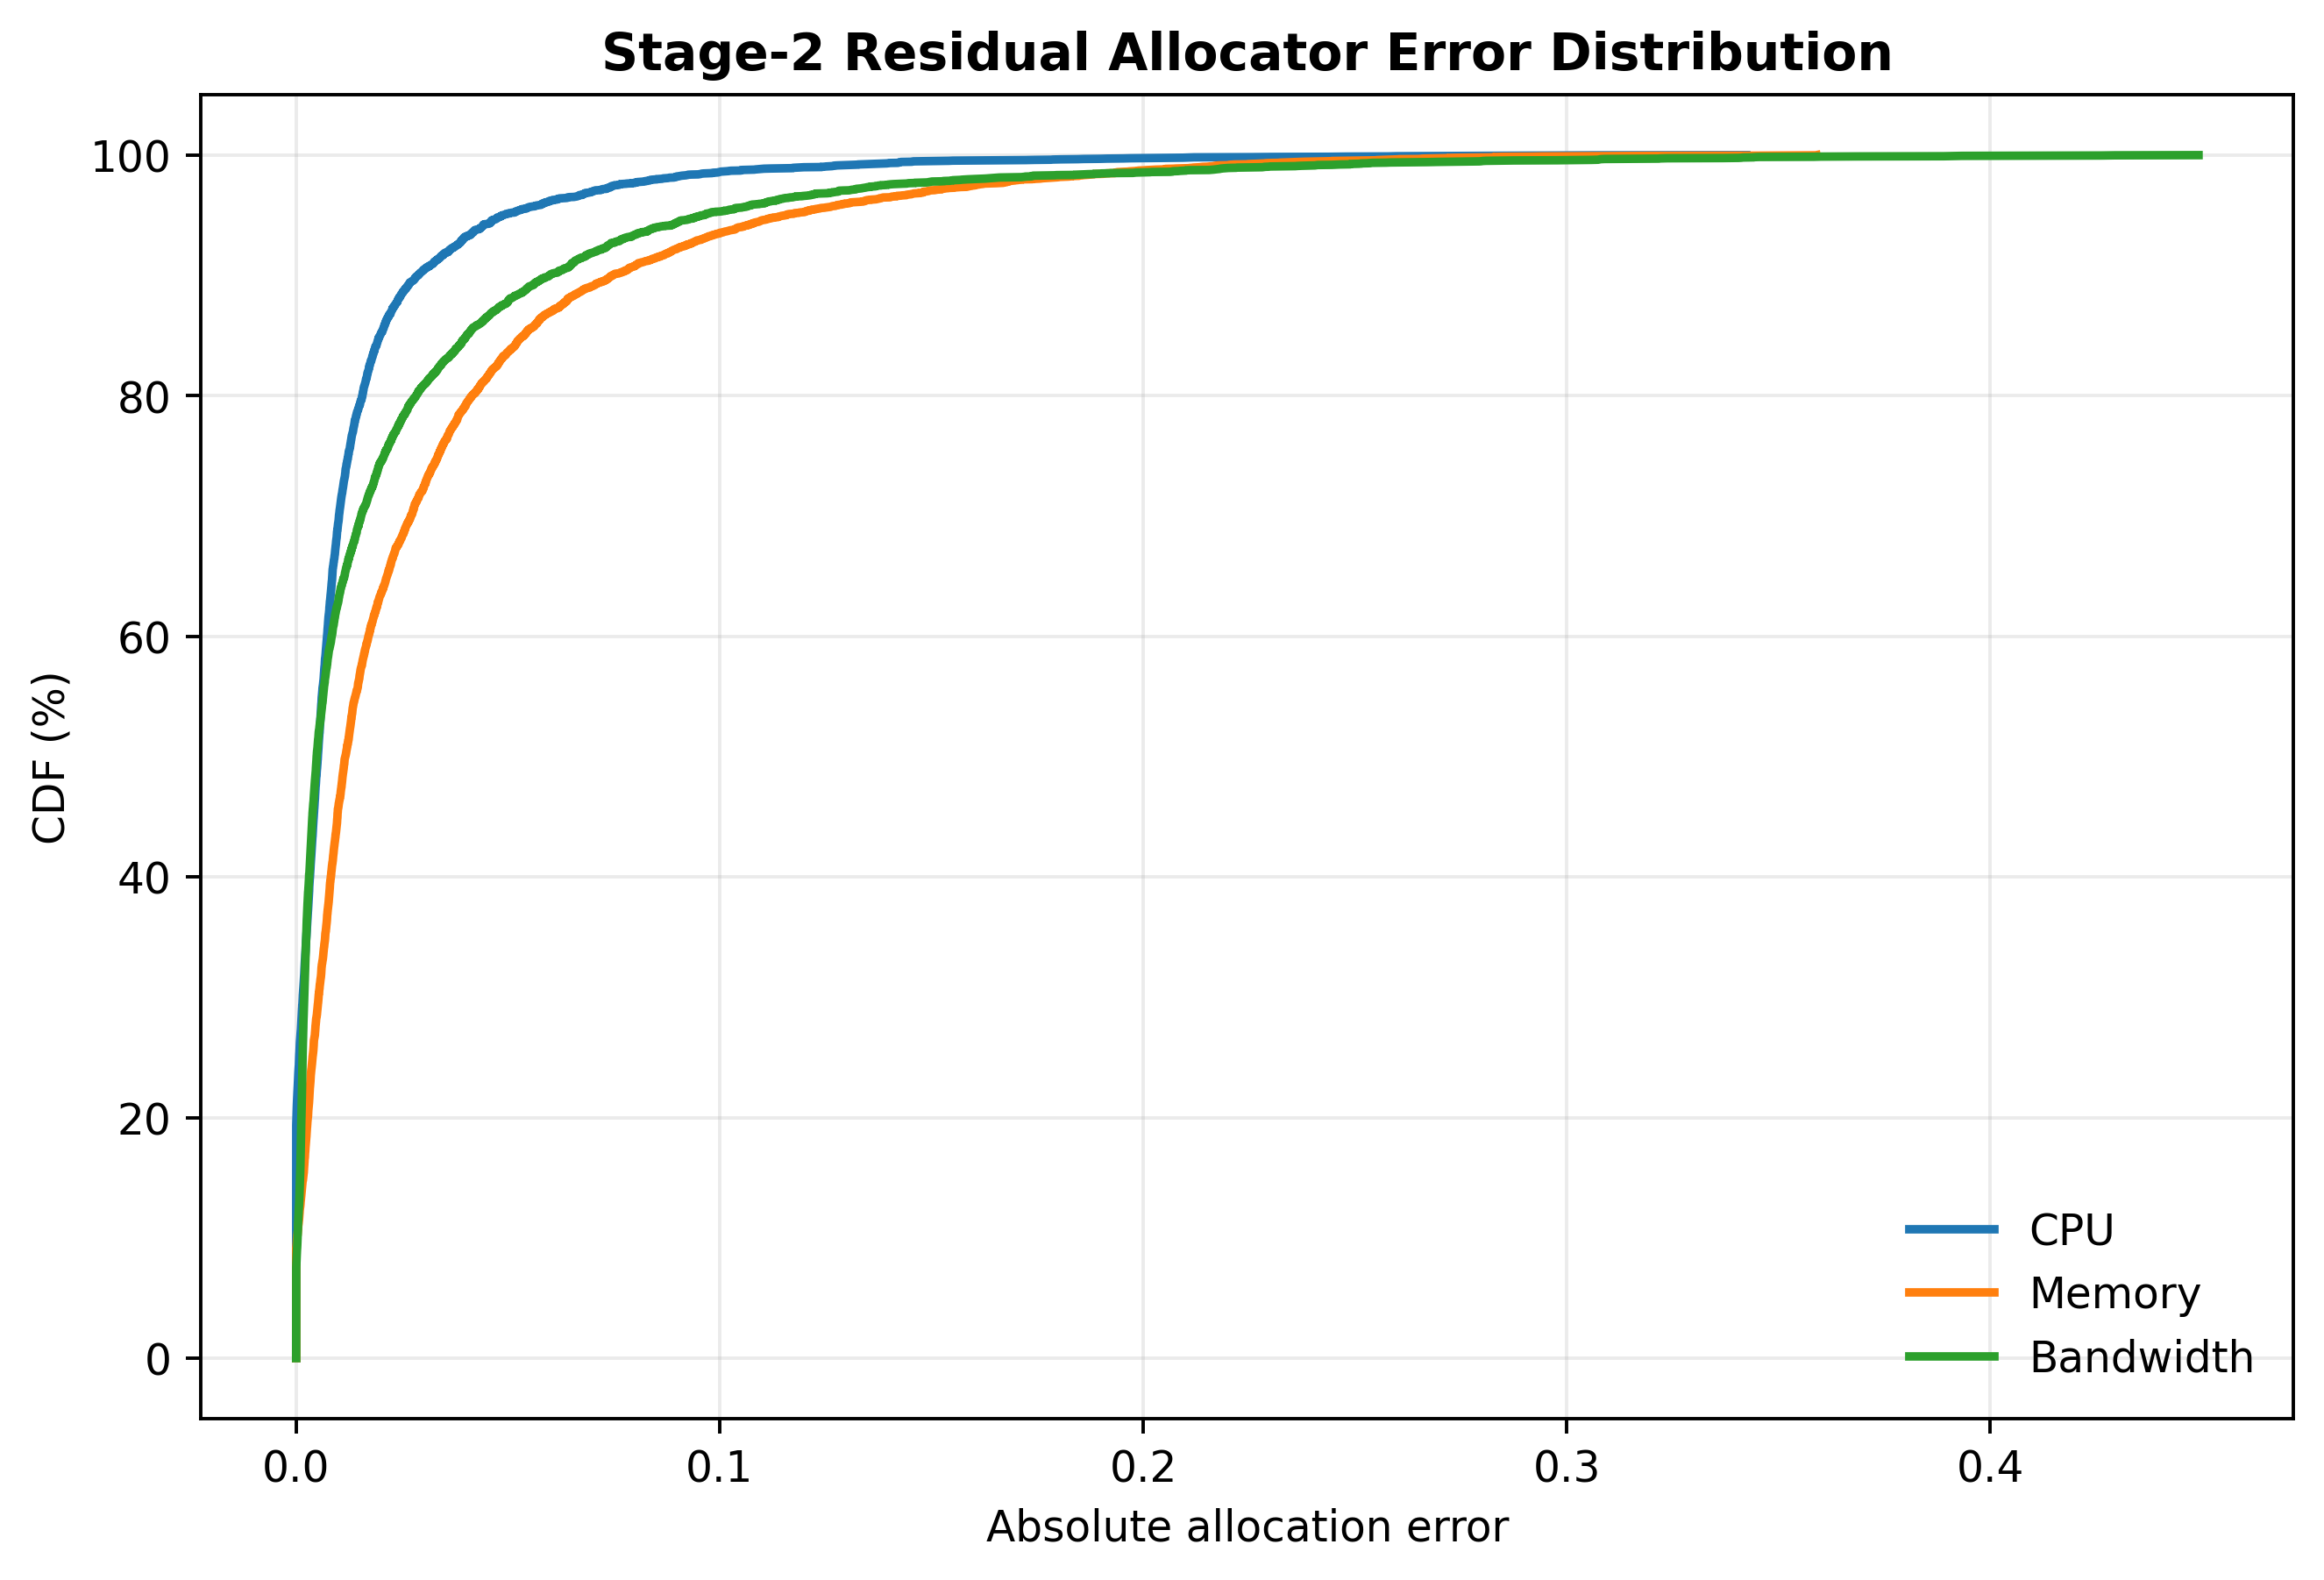
\includegraphics[width=0.92\columnwidth]{figures/diagnostics/167_fig_a20_allocator_resource_error_cdf.png}
\caption{CDF of proxy-target resource-allocation error. Capacity normalization and risk projection reduce the high-error tail relative to raw residual output.}
\label{fig:allocator_cdf_main}
\end{figure}

Figure~\ref{fig:allocator_cdf_main} should be read together with
Fig.~\ref{fig:allocator_projection_readout}. The CDF shows that most resource
errors are small after residual correction, while the projection equation
explains how the final assignment is kept inside the feasible capacity region.
This is the main reason the residual allocator is reported with both accuracy
and feasibility metrics: low prediction error is useful only when the assigned
CPU, memory, and bandwidth remain admissible for the selected edge node.

The practical reading is straightforward. Demand-proportional allocation gives a
stable starting point, the residual model adjusts for deadline and priority
conditions, and the risk term protects tasks that are likely to miss QoS after
edge selection. Capacity projection then prevents the learned correction from
turning into an infeasible assignment during high-load intervals.

\begin{table*}[!t]
\centering
\caption{Stage-2 allocator proxy-target error and feasibility on $\mathcal{I}^{\mathrm{valid}}_e$, the Fed-DDQN edge-selected allocator-valid test subset.}
\label{tab:allocator_results}
\small
\setlength{\tabcolsep}{5pt}
\begin{tabular}{@{}lrrrr@{}}
\toprule
Method & Overall MAE & Underalloc. (\%) & Waste (\%) & Cap. viol. (\%) \\
\midrule
Equal Allocation & 0.3030 & 16.59 & 57.01 & 0.00 \\
Demand-Proportional & 0.0656 & 23.56 & 16.93 & 0.00 \\
Priority-Weighted & 0.2808 & 10.89 & 47.09 & 0.00 \\
Deadline-Aware & 0.3268 & 23.06 & 52.60 & 0.00 \\
Rejection-Aware Demand & \textbf{0.0196} & 6.98 & \textbf{5.46} & 0.00 \\
Residual Allocator Raw & 0.0504 & 11.39 & 19.24 & 35.16 \\
Residual + Capacity Norm & 0.0366 & 15.23 & 12.12 & 0.00 \\
Residual + Risk Projection & 0.0204 & \textbf{6.65} & 5.75 & \textbf{0.00} \\
\bottomrule
\end{tabular}
\end{table*}

\begin{table*}[!t]
\centering
\caption{Stage-2 allocator proxy-target and QoS-oriented comparison on the allocator-valid edge-selected subset.}
\label{tab:allocator_qos}
\small
\setlength{\tabcolsep}{5pt}
\begin{tabularx}{\textwidth}{@{}lrrX@{}}
\toprule
Method & Est. SLA risk (\%) & Efficiency & Interpretation \\
\midrule
Equal Allocation & 4.57 & 58.319 & Balanced but wastes resource because task demand is ignored. \\
Demand-Proportional & 5.96 & 66.692 & Low error relative to simple baselines, but under-allocation remains high. \\
Priority-Weighted & 3.31 & 68.623 & Reduces risk for urgent tasks but wastes more resource. \\
Deadline-Aware & 3.12 & 54.338 & Protects deadlines but over-allocates and loses efficiency. \\
Rejection-Aware Demand & 3.55 & 89.062 & Best MAE and waste, using the hand-designed risk-aware demand rule. \\
Residual Allocator Raw & 4.08 & 57.773 & Neural residual learns useful corrections but violates capacity before projection. \\
Residual + Capacity Norm & 3.61 & 78.120 & Removes capacity violations and improves feasibility. \\
Residual + Risk Projection & 3.50 & \textbf{89.295} & Best efficiency, lowest under-allocation, and zero capacity violation. \\
\bottomrule
\end{tabularx}
\end{table*}


\FloatBarrier
\subsection{Discussion}

The results support the proposed two-stage structure. \fedddqn{} is the main contribution because it improves the edge/cloud scheduling decision on the benchmark dataset. The allocator is a secondary contribution because it improves proxy-target allocation fit for the allocator-valid edge-selected subset after the scheduler has already acted. Keeping these roles separate makes the result easier to interpret.

The result also shows the value of \dataset{}. The scenario-wise and workload-timeline figures indicate that the policy is exposed to bursts, congestion, outage, and resource variation. This stress structure makes the benchmark suitable for comparing offloading policies under repeatable but demanding conditions.

Finally, the latency-reference Oracle gap identifies directions for future optimization. The learned policy remains about 12.7 ms above that generated latency reference, leaving room for recurrent policies, graph-based edge-state encoders, and online state mutation where policy actions affect subsequent queues directly.

\subsection{Interpretation and Practical Implications}

The proposed federated DDQN configuration achieves the best average latency among the main comparison methods in Table~\ref{tab:main_results} while keeping rejection and SLA behavior close to the reported Oracle values. This combination matters for edge-cloud IoT scheduling because a policy must reduce delay without shifting difficult tasks into rejection or overloading one execution tier.

The main qualitative result is the reduction of edge bias. Deadline-heavy workloads can make a policy route too many tasks to edge, which helps emergency tasks but hurts AI, video, image, and firmware-like cases. The reward and validation design bring edge usage closer to the Oracle level. That is why the paper reports edge usage, scenario behavior, and Oracle agreement rather than only latency. The method is not simply using one destination more often.

The allocator result follows the same staged logic. Residual learning improves proxy-target allocation fit on the allocator-valid edge-selected subset, and the best allocator result comes from combining learned correction with risk projection and normalization. For resource management, the constrained final prediction is preferable because it keeps the allocation feasible while improving proxy-target error and QoS-oriented efficiency.
